\documentclass{note}
\usepackage[cpp,table,pseudo]{mypackage}
\usepackage{footnote}
\makesavenoteenv{tabular}

\def\ojoin{\setbox0=\hbox{$\bowtie$}%
  \rule[-.02ex]{.25em}{.4pt}\llap{\rule[\ht0]{.25em}{.4pt}}}
\def\leftouterjoin{\mathbin{\ojoin\mkern-5.8mu\bowtie}}
\def\rightouterjoin{\mathbin{\bowtie\mkern-5.8mu\ojoin}}
\def\fullouterjoin{\mathbin{\ojoin\mkern-5.8mu\bowtie\mkern-5.8mu\ojoin}}

\renewcommand{\thefootnote}{\fnsymbol{footnote}}
\lstset{language=sql}

\title{数据库系统原理笔记}
\author{陈鸿峥}
\date{{\builddatemonth\today}\protect\footnote{\text{Build \builddate\today}}} % protect!

\begin{document}

\maketitle
\renewcommand{\thefootnote}{\arabic{footnote}}
\setcounter{footnote}{0}

\setcounter{tocdepth}{2}%设置深度
\tableofcontents

\bigskip\bigskip

% !TEX root = main.tex

\section{计算机系统概述}
\subsection{计算模型}
\begin{itemize}
	\item 图灵机(1936)
	\item 冯诺依曼体系结构(1945)\footnote{非冯诺依曼体系结构:并行计算、量子计算、生物计算} --- 存储程序原理(\textbf{运算器}为中心)\\
	计算机采用\textbf{二进制}表示机器指令和数据,按照程序指令\textbf{顺序}执行
\begin{center}
\begin{tikzcd}
& & \text{存储器}\arrow{d} & & \\
\quad\arrow{r} & \text{输入设备}\arrow{r} & \text{运算器}\arrow{r}\arrow{d}\arrow{u} & \text{输出设备}\arrow{r} & \quad\\
& & \text{控制器}\arrow{u}\arrow{lu}\arrow{ru}\arrow[bend left]{uu} & &
\end{tikzcd}
\end{center}
而现在由于计算不是瓶颈,存储访问成为了瓶颈,故现代微机以\textbf{存储器}为中心
\begin{center}
\begin{tikzcd}
& & \text{运算器}\arrow{d} & & \\
\quad\arrow{r} & \text{输入设备}\arrow{r} & \text{存储器}\arrow{r}\arrow{d}\arrow{u} & \text{输出设备}\arrow{r} & \quad\\
& & \text{控制器}\arrow{u}\arrow{lu}\arrow{ru}\arrow[bend left]{uu} & &
\end{tikzcd}
\end{center}
\end{itemize}
[运算器、控制器](CPU)、存储器为计算机的核心,合称主机;外围设备,简称外设,指除主机外的其他设备,包括IO设备、外存等

计算机中的信息仍用二进制表示的原因:由物理器件性能决定
\begin{itemize}
	\item 二进制只有两种状态,容易找到具有2个稳定状态并且状态转换容易控制的物理器件(数字电路)
	\item 二进制编码运算规则简单
	\item 二进制的0、1与二值逻辑一致,容易实现逻辑运算
\end{itemize}
% There are two reasons computers use the binary system:
% 1.Two clearly distinct states that provide a safety range for reliability.
% 2.Least amount of necessary circuitry, which results in the least amount of space, energy consumption, and cost.

\subsection{计算机的发展历程}
按发展历程可分为:电子管、晶体管、集成电路、(超)大规模集成电路四代计算机
\par重大历史事件如下
\begin{center}
\begin{tabular}{|c|c|c|c|}
\hline
% 年份 & 姓名 & 事件 & 备注 \\
1904 & 弗莱明(Fleming) & 二极管 & \\\hline
1907 & 德福雷斯特(De Forest) & 三极管 & \\\hline
1938 & 香农(Shannon) & 布尔代数与二值电子器件(继电器) & 奠定数字电路基石 \\\hline
1946 & & 第一台通用计算机ENIAC & 十进制 \\\hline
1947 & \begin{tabular}{c}布莱顿(Brattain)\\
巴丁(Bardeen)\end{tabular} & 点接触晶体管 & \\\hline
1949 & 肖克利(Shockley) & 结型晶体管(1949) & 1956诺贝尔奖\\\hline
1950 & & 二进制和存储程序EDVAC & 实现冯诺依曼设想(组合进步) \\\hline
1958 & Jack Kilby & 集成电路 & 2000诺贝尔奖 \\\hline
1965 & Moore & 摩尔定律 & \begin{tabular}{c}
在价格不变的情况下,每18个月芯片上\\
晶体管数目翻倍,性能也提升一倍
\end{tabular}\\\hline
1971 & Intel & 第一款微处理器4004 & 10$\mu$m\\\hline
\end{tabular}
\end{center}

\subsubsection{单处理器(1971-2002)}
性能提升主要手段
\begin{itemize}
	\item 提升工作主频:KHz增长至GHz(生产工艺进步,流水线级数增加)
	\item 指令级并行(ILP)
\end{itemize}
\begin{proposition}[安迪-比尔定律]
Andy gives, Bill takes away. 安迪是原Intel CEO,比尔是原微软CEO,硬件厂商靠软件开发商用光自己提供的硬件资源得以生存
\end{proposition}
但遇到频率墙和功耗墙
\[\text{功耗(power)}\propto 1/2\times\text{CMOS电容}\times\text{电压}^2\times\text{转换(01)频率}\]
\par
2004年,Intel放弃4GHz Pentium4芯片开发,因无法解决散热问题,通过加快主频提升处理器性能的路走到尽头

\subsubsection{多核处理器(2005-)}
采用多核处理器不过是将硬件的问题丢到软件\footnote{“向多核的转变并不是因为我们在软件或体系结构技术上取得了中大突破而带来的。相反,这种转变是当单处理器体系结构发展遇到了难以克服的巨大障碍时,我们被迫作出的一种选择。”---Kurt Keutzer (UCB), \emph{The Landscape of Parallel Computing Research: A View from Berkeley}}
\begin{theorem}[阿姆达尔(Amdahl)定律]
\label{thm:amdahl}
\[\text{改进后的执行时间}=\text{受改进影响部分的执行时间}/\text{改进提高的倍数}+\text{不受影响的执行时间}\]
\[S_A=\frac{1}{s+(1-s)/N},\]
\end{theorem}
对计算机系统的某个部分采用并行优化措施后所获得的计算机性能的提高是有上限的,上限由串行部分所占的比例决定
\begin{theorem}[古斯塔夫森(Gustafson)定律]
\[S_G=(s'+p'\times N)/(s'+p')=N+(1-N)\times s',\]
其中,$s'$和$p'$为程序串行部分与可并行化部分在并行系统上执行的时间占总时间的比例,$N$为处理器数量,简便起见设总时间$s'+p'=1$
\end{theorem}
打破Amdahl定律\textbf{问题规模不变}的假设,任何足够大的任务都可以被有效地并行化,只要问题规模可扩展,并行所带来的加速比就可以扩展


\subsection{计算机系统的层次结构}
\begin{center}
\begin{tikzcd}
\text{高级语言层}\arrow{d}{}\\
\text{汇编语言层}\arrow{d}{}\\
\text{操作系统层}\arrow{d}{}\\
\text{指令系统层}\arrow{d}{}\\
\text{微体系结构层}\arrow{d}{}\\
\text{数字逻辑层}
\end{tikzcd}
\end{center}
程序编译运行过程:
\begin{center}
\begin{tikzcd}
\text{高级语言}\quad\arrow{r}{\text{预编译、编译}} & \quad\text{汇编语言}\arrow{r}{\text{汇编}} & \text{目标文件(二进制)}\arrow{r}{\text{链接}} & \text{可执行文件(二进制)}\arrow{d}{\text{加载}}\\
& & \text{电路上的电信号}\quad & \quad\text{二进制机器指令流(硬盘$\to$存储器)}\arrow[swap]{l}{\text{CPU取指译码}}
\end{tikzcd}
\end{center}
计算机内部工作过程:逐条执行加载到内存中的二进制机器指令流的过程

指令执行分为两个阶段,周期性重复性进行:
\begin{itemize}
	\item 取指阶段:CPU从内存中读取指令,程序计数器(PC)保存要被要被取出的\textbf{下一条}指令的地址,除非遇跳转指令,否则都加一个增量\footnote{程序计数器(Program Counter)是一个实际存在的寄存器吗? - Belleve的回答 - 知乎 \url{https://www.zhihu.com/question/22609253/answer/21965180} PC每次增加\textbf{一条指令的长度/寻址粒度},在MIPS中一条指令长4字节,寻址粒度1字节,故每次PC加4;而x86体系指令长度不定,每次增加量会变化}
	\item 执行阶段:对取出的指令译码后执行
\end{itemize}
软件系统可分为系统软件和应用软件

\subsection{计算机结构的八个想法}
\begin{enumerate}
	\item 摩尔(Moore)定律:集成电路资源每$18-24$个月翻倍
	\item 抽象(abstraction):简化设计
	\item 加速常用操作(Make common case fast):见定理\ref{thm:amdahl}
	\item 并行(parallelism)
	\item 流水线(pipelining)
	\item 预测(prediction)
	\item 内存等级制(hierarchy)
	\item 冗余实现可靠性(redundancy):检测故障及解决
\end{enumerate}

\subsection{基本指标}
表示计算机通信带宽时
\begin{center}
\begin{tabular}{ccccccc}\hline
KB(yte) & MB & GB & TB & PB & EB & ZB\\\hline
$10^3$ & $10^6$ & $10^9$ & $10^{12}$ & $10^{15}$ & $10^{18}$ & $10^{21}$\\\hline
\end{tabular}
\end{center}
表示计算机存储二进制时
\begin{center}
\begin{tabular}{ccccccc}\hline
KiB(yte) & MiB & GiB & TiB\\\hline
$2^{10}$ & $2^{20}$ & $2^{30}$ & $2^{40}$\\\hline
\end{tabular}
\end{center}
\begin{itemize}
	\item 位(bit/b):计算机处理、存储、传输信息的最小单位
	\item 字节(Byte/B) $1\text{ Byte}=8\text{ bit}$:现代计算机主存按字节编制,字节是最小可寻址单位
	\item 字(Word):表示被处理信息的单位,用来度量数据类型的宽度\footnote{字长是指CPU中\textbf{数据通路的宽度},等于CPU内部总线的宽度或运算器的位数或通用寄存器的宽度;字和字长的宽度可以一样,也可以不同,通常是字节的整数倍}
\end{itemize}
\par 一台32位的电脑,一个字等于4个字节,字长为32位;若字长为16位,则一个字等于2字节.
\par 4字节相当于8位16进制编码

\subsection{性能评价}
\label{subsec:performance}
CPU主频:对同一型号计算机,主频越高,完成指令一个执行步骤时间越短
\[\text{计算机的性能(Performance)}=1/\text{执行时间(Execution time)}\]
按照单位(量纲)进行换算即可
\[\begin{aligned}
\text{CPU执行时间(s)}&=\text{执行程序所需CPU时钟周期(cyc)}\times\text{时钟周期s/cyc)}\\
&=\text{指令数目(ins)}\times\text{CPI(cyc/ins)}\times\text{时钟周期(s/cyc)}
\end{aligned}\]
程序性能对执行事件的影响:
\begin{center}
\begin{tabular}{|c|c|c|c|}\hline
 & 指令数 & CPI & 时钟周期\\\hline
算法、编程语言、编译器 & $\times$ & $\times$ & \\\hline
指令集 & $\times$ & $\times$ & $\times$ \\\hline
计算机组成 & & $\times$ & $\times$ \\\hline
实现技术 & & & $\times$\\\hline
\end{tabular}
\end{center}
体系结构=指令集体系结构(功能定义与设计)+计算机组成(考虑用什么材料)\\
举例来说:
\begin{itemize}
	\item 指令集(ISA)考虑:是否提供乘法指令
	\item 组成(Organization)考虑:如何实现乘法指令(专门乘法器还是加法器+移位器)
	\item 实现技术(Technology)考虑:如何布线、用什么材料和工艺
\end{itemize}

% 带有处理器的设备一般称为智能化设备
% 完整的计算机系统应包括配套的硬件设备和软件系统
% !TEX root = main.tex

\section{SQL简介} % Chap 3
SQL即结构化查询语言(Structured Query Language, SQL)

\subsection{数据定义语言(DDL)}
数据类型
\begin{itemize}
	\item \verb'char(n)':固定长度字符串
	\item \verb'varchar(n)':可变长度字符串,用得最多
	\item \verb'int'
	\item \verb'smallint'
	\item \verb'numeric(p,d)':定点数,共$p$位(包括符号位),其中$d$位在小数点右侧
	\item \verb'real', \verb'double precision'
	\item \verb'float(n)':精度至少为$n$位的浮点数
\end{itemize}
\begin{lstlisting}[language=sql]
create table instructor (
	ID char(5),
	name varchar(20) not null,
	dept_name varchar(20),
	salary numeric(8,2) default 0,
	primary key (ID), -- integrity constraints
	foreign key (dept_name) references department);
\end{lstlisting}

\subsection{数据查询语言}
基本的形式如下所示
\begin{lstlisting}[language=sql]
select A1, A2, ..., An
from r1, r2, ..., rm
where P
\end{lstlisting}
其中$A_i$为属性(attribute)、$R_i$为一个关系(relation)/一个表、$P$是谓词(preicate),返回满足关系的数组。

\begin{itemize}
	\item 自然连接(natural join):将两个关系的各个元组进行连接,并且只考虑那些在两个关系模式中\textbf{都出现}的属性上取值相同的元组对(相当于取\textbf{交})
	\item 连接(join):用\verb'using'可以只考虑某一特定属性的连接
\end{itemize}
\begin{lstlisting}[language=sql]
select name, title
from (instructor natural join teachers) join course using (course_id);
-- only join two relations with the same course_id
\end{lstlisting}

字符串运算:模式匹配
\begin{itemize}
	\item \verb'upper(s)'、\verb'lower(s)'
	\item \verb'%':匹配任意字串
	\item \verb'_':匹配任意一个字符
	\item \verb'like':以这些字符串进行匹配
\end{itemize}

\begin{lstlisting}[language=sql]
select distinct dept_name
from instructor

select * -- all attributes
from instructor

select '437' as FOO

select ID, name, salary/12 as monthly_salary

select name
from instructor
where dept_name = 'Comp. Sci.' and salary > 80000

select *
from instructor, teaches -- Cartesian product

select distinct T.name
from instructor as T, instructor as S -- rename, Cartesian product
where T.salary > S.salary and S.dept_name = 'Comp. Sci.'
-- salary between 90000 and 100000

/**
percent ( % ). The % character matches any substring.
underscore ( _ ). The _ character matches any character.
**/
select name
from instructor
where name like '%dar%' matches any string containing "dar" as a substring

select distinct name
from instructor
order by name -- sorted

select *
from instructor
order by salary desc, name asc;

(select course_id from section where sem = 'Fall' and year = 2017)
union -- intersect, except
(select course_id from section where sem = 'Spring' and year = 2018)

select name
from instructor
where salary is null

-- aggregrate functions
-- arg, min, max, sum, count
select dept_name, avg (salary) as avg_salary
from instructor
where dept_name= 'Comp. Sci.'
group by dept_name;

select count (distinct ID)
from teaches
where semester = 'Spring' and year = 2018;

-- group constraints
-- find the average salary in each dept
select dept_name, avg(salary) as avg_salary
from instructor
group by dept_name -- can only be contained by select clause
having avg(salary) > 42000; -- effected after grouping
\end{lstlisting}

注意对于简单问题,通常没有必要用嵌套子查询,直接开几个关系即可
\begin{example}
对于下列两个关系表
\begin{itemize}
	\item Book(BID,title,AID,subject)
	\item Author(AID,first\_name,last\_name)
\end{itemize}
找出所有写了至少两种subject的作者的名字
\end{example}
\begin{analysis}
直接创建两个Book关系
\begin{lstlisting}
select a.last_name, a.first_name
from author a, book b1, book b2
where b1.aid = a.aid and b2.aid = a.aid and b1.subject != b2.subject
\end{lstlisting}
\end{analysis}

三值逻辑,添加了Unknown(其实就是T/F都恒成立的关系才会输出正常值)
\begin{center}
\begin{tabular}{|c|c|c|}\hline
AND & OR & NOT\\\hline
\begin{tabular}{l}
$T \land U = U$\\
$F \land U = F$\\
$U \land U = U$
\end{tabular} & 
\begin{tabular}{l}
$T \lor U = T$\\
$F \lor U = U$\\
$U \lor U = U$
\end{tabular} &
$\lnot U = U$\\\hline
\end{tabular}
\end{center}

SQL在谓词中使用\verb'null'测试空值,因而为找出\verb'instructor'关系中\verb'salary'为空值的所有教师,可写
\begin{lstlisting}
select name
from instructor
where salary is null
\end{lstlisting}

集合成员资格通过\verb'in'来判断,同时有\verb'some'和\verb'all'的关系测试,下面给出了一些嵌套子查询的例子。
\begin{lstlisting}
select name
from instructor
where salary > some (select salary
					from instructor
					where dept_name = 'Biology')

select S.ID, S.name
from student as S
where not exists ((select course_id
				from course
				where dept_name = 'Biology')
				except
				(select T.course_id
				from takes as T
				where S.ID = T.ID))

select T.course_id
from course as T
where 1 >= (select count(R.course_id)
			from section as R
			where T.course_id = R.course_id and R.year = 2009);
-- there is no unique in MySQL

with max_budget(value) as
	(select max(budget)
	from department)
select budget
from department, max_budget
where department.budget = max_budget.value;

select dept_name,
	(select count(*)
	from instructor
	where department.dept_name = instructor.dept_name)
	as num_instructors
from department; -- scalar subquery
\end{lstlisting}

数据库的修改操作如下
\begin{lstlisting}
delete from instructor
where dept_name = 'Finance';

insert into course(course_id, title)
	values ('CS-437','Database Systems');

update instructor
set salary = salary * 1.05
where salary < 70000;

update instructor
set salary = case
			when salary <= 1000 then salary * 1.05
			when salary <= 2000 then salary * 2.05
			else salary * 1.03
		end
\end{lstlisting}
% !TEX root = main.tex

\section{进阶SQL} % Chap 4
\subsection{内外连接}
\verb'on'条件可以提供比自然连接更为丰富的连接条件
\begin{lstlisting}
select *
from students join takes on student.ID = takes.ID; -- condition
\end{lstlisting}

直接使用\verb'natural join'可能导致元组丢失,比如有一些学生没有选修任何课程,则其在student关系中不会与takes关系中任何元组配对。
因此有\textbf{外连接}:
\begin{itemize}
	\item 左外连接(left outer join):只保留出现在左外连接运算之前(左边)关系中的元组,若右侧关系中没有对应属性则用null代替
	\item 右外连接(right outer join)
	\item 全外连接(full outer join):左外连接和右外连接的组合
\end{itemize}

从而可以很容易查询出“所有课程一门也没有选修的学生”:
\begin{lstlisting}
select ID
from student natural left outer join takes
where course_id is null;
\end{lstlisting}

为了将常规连接和外连接区分开,SQL中将常规连接称为内连接(inner join),默认的都是内连接。

\subsection{视图}
让用户看到整个逻辑模型显然是不合适的,出于安全考虑,可能需要向用户隐藏特定的数据。
本来通过select可以把需要的数据计算并存储下来,但一旦底层数据发生变化,查询的结果就不再匹配。
因此,为了解决这样的问题,SQL提供一种虚关系,称为视图(view),只有在使用的时候才会被计算。
\begin{lstlisting}
create view faculty as
select ID, name, dept_name
from instructor;
\end{lstlisting}
之后便可以直接使用\verb'from'语句访问视图。

\begin{definition}[物化视图(materialized view)]
如果用于定义视图的实际关系改变,视图也会跟着修改。
\end{definition}

由于视图并不是数据库底层的关系,故一般数据库不允许对视图关系进行修改。

\subsection{事务}
SQL标准规定当一条SQL语句被执行,就隐式开始了一个事务。
下列SQL语句之一会结束一个事务:
\begin{itemize}
	\item Commit work:将事务所做的更新在数据库中持久保存。
	在事务被提交后,一个新的事务自动开始。
	\item Rollback work:撤销该事务中所有SQL语句对数据库的更新,数据库将恢复到执行该事务的第一条语句之前的状态。
	如果遇断电,回滚会在下一次重启时自动执行。
\end{itemize}

\subsection{完整性约束}
单个关系上的约束
\begin{itemize}
	\item \verb'not null':跟在属性定义后面
	\item \verb'unique (A1,A2,...,Am)':声明$A_1,\ldots,A_m$构成一个候选码
	\item \verb'check(<predicate>)':关系中每个元组都必须满足该谓词,如\verb'check(budget>0)'
\end{itemize}

参照完整性/子集依赖:外码
\begin{lstlisting}
foreign key (dept_name) references department
	on delete cascade
	on update cascade
\end{lstlisting}
会级联(cascade)删除或更新。

\subsection{授权}
\verb'grant'授权,\verb'revoke'回收
\begin{itemize}
	\item \verb'select':允许用户修改关系中任意数组
	\item \verb'insert'
	\item \verb'delete'
\end{itemize}
用户名\verb'public'包括了当前所有用户和未来用户的权限。

\begin{lstlisting}
grant <authorization list>
on <relation name/view name>
to <user/user list>

grant update (budget) on department to Amit, Satoshi;
\end{lstlisting}

可以先创建角色(role)然后给用户授予角色。
% !TEX root = main.tex

\section{形式化关系查询语言} % Chap 6
\subsection{关系代数}
\begin{center}
\begin{tabular}{|c|c|c|}
\hline
选择 & $\sigma$ &
\begin{tabular}{l}
挑选出符合一定性质的元组\\
$\sigma_{\text{Sub="Phy"}\land\text{age}>30}(\text{teachers})$
\end{tabular}\\\hline
投影 & $\Pi$ & 
\begin{tabular}{l}
只选出对应属性\\
$\Pi_{\text{ID,name,salary}}(\text{teachers})$
\end{tabular}\\\hline
笛卡尔积 & $\times$ & 将两个关系整合(简单并置,需要进一步筛选)\\\hline
自然连接 & $r\Join s=\prod_{R\cup S}(\sigma_{r.A_1=s.A_1\land\cdots\land r.A_n=s.A_n})(r\times s)$ & \\\hline
$\theta$连接 & $r\Join_\theta s=\sigma_\theta(r\times s)$ & \\\hline
外连接 & $\leftouterjoin, \rightouterjoin, \fullouterjoin$ & \\\hline
并集 & $\cup$ & 数目应相同,属性可兼容\\\hline
交集 & $\cap$ & \\\hline
差集 & $-$ & \\\hline
赋值 & $\gets$ & \\\hline
重命名 & $\rho_x(E)$ & 给$E$的返回值赋名为$x$\\\hline
\end{tabular}
\end{center}

扩展的关系代数运算:
\begin{itemize}
	\item 广义投影:$\prod_{F_1,F_2,\ldots,F_n}(E)$,其中$F_i$中每一个都是涉及常量及$E$的模式中属性的算术表达式
	\item 聚类:$\mathcal{G}$,如count, min, max,考虑group by可以写成下列形式
	\[{}_{dept\_name}\mathcal{G}_{\textbf{average}(salary)}(instructor)\]
\end{itemize}

\begin{definition}[聚集运算]
聚集运算$\mathcal{G}$的通常形式如下:
\[{}_{G_1,G_2,\ldots,G_n}\mathcal{G}_{F_1(A_1),\ldots,F_n(A_n)}(E)\]
其中$E$是任意关系代数表达式,$G_1,\ldots,G_n$是用于分组的一系列属性;
每个$F_i$是一个聚集函数,每个$A_i$是一个属性名。
$E$结果中的元组将会以如下方式分为若干组:
\begin{itemize}
	\item 同组中所有元组在$G_1,\ldots,G_n$上的取值相同
	\item 不同组中的元组在$G_1.\ldots,G_n$上的取值不同
\end{itemize}
\end{definition}

\subsection{其他关系演算}
\subsubsection{元组关系演算}
元组关系演算是非过程化的查询语言(有点像声明式语言),它只描述所需信息,而不给出获得该信息的具体过程。
查询表达为
\[\{t\mid P(t)\}\]
即使谓词$P$为真的元组$t$的集合,$t[A]$表示元组$t$在属性$A$上的值,用$t\in r$表示元组$t$在关系$r$中。

如工资大于80000美元的所有教师的ID为(注意这里涉及到属性选择)
\[\{t\mid\exists s\in instructor(t[ID]=s[ID]\land s[salary]>80000\}\]

其实与命题逻辑类似
\[t\in\text{instructor}\land\exists s\in\text{department}(t[\text{dept\_name}]=s[\text{dept\_name}])\]
前者$t$为自由变量,后者$s$为受限变量。

元组关系演算可能产生一个无限的关系
\[\{t\mid\lnot(t\in instructor)\}\]
这样的元组有无限多个且不在数据库中,因此这样写是\textbf{不安全的}。

因此引入元组关系公式$P$的域的概念,如$\dom(t\in instructor\land t[salary]>80000)$是包括80000和出现在instructor中的所有值集合。
若表达式$\{t\in P(t)\}$结果所有值均来自$\dom(P)$,则说表达式$\{t\in P(t)\}$是安全的。

\subsubsection{域关系演算}
\[\{<x_1,x_2,\ldots,x_n>\mid P(x_1,x_2,\ldots,x_n)\}\]
其中$<x_1,\ldots,x_n>\in r$,每一个$x_i$为域变量,$r$为$n$个属性上的关系。

与元组关系演算最大的区别在于,域关系演算更加细粒度。
比如找出工资大于80000美元的所有教师的ID:
\[\{<i>\mid\exists n,d,s(<i,n,d,s>\in instructor\land s>80000)\}\]

同样有安全性问题,可类似定义。
% !TEX root = main.tex

\section{E-R模型} % Chap 7
在设计一个数据库模式时,要避免以下两个缺陷:
\begin{itemize}
	\item 冗余:可能导致不同关系表中的信息没有及时更新
	\item 不完整:只有对应开课的实体而没有对应课程的实体
\end{itemize}

\subsection{实体-关系模型}
\begin{definition}[实体]
实体是现实世界中可区别于所有其他对象的一个事物或对象。
每个实体有一组性质/属性(attribute),其中一些性质的值可以唯一标识一个实体。
实体集则是相同类型具有相同属性或性质的一个实体集合。
实体集是一个抽象概念,而实体集的外延(extension)则是指属于实体集实体的实际集合。
\end{definition}

大学中实际教师的集合构成了实体集instructor的外延。
实体集不必互不相交,如定义大学里所有人的实体集(person)。
一个person实体可以是instructior实体,可以是student实体,可以既是instructor实体又是student实体,也可以都不是。

\begin{definition}[联系]
联系(relationship)是指多个实体间的相互关联。
联系集是相同类型联系的集合。
\[\{(e_1,e_2,\ldots,e_n)\}\mid e_1\in E_1, e_2\in E_2, \ldots, e_n\in E_n\]
联系也可以具有\underline{描述性属性}(如下右图)。
\begin{figure}[H]
\centering
\begin{tabular}{cc}
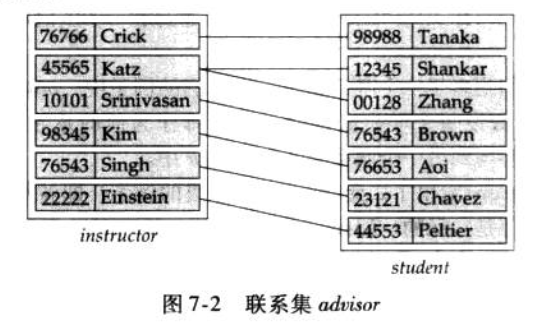
\includegraphics[width=0.5\linewidth]{fig/relationship_set.png}
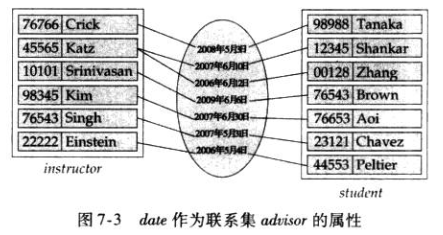
\includegraphics[width=0.5\linewidth]{fig/relationship_set(description).png}
\end{tabular}
\end{figure}
实体集之间的关联称为参与(participation),若$E$中每个实体都参与到联系集$R$中的至少一个联系中,则称参与是全部的(total)的,否则是部分的(partial)。
E-R模式中的联系实例则为具体命名实体间的关联。
实体在联系中扮演的功能称为实体的角色(role)。
参与联系集的实体集数目称为联系集的度(degree),二元联系集的度为2,三元联系集度为3。
\end{definition}

\begin{definition}[属性]
每个属性都有一个可取值的集合,称为该属性的域(domain),或值集(value set)。
属性可以分为简单和复合(composite)属性,复合属性可以再划分为更小的部分,如名字分为名和姓。
也可能是单值或多值属性,比如老师可以有多个电话号码,这是多值属性。
还有派生(derived)属性,可以通过其他属性计算得出。
\end{definition}
通常如果一个属性在两个实体集中出现,且这两个实体集存在关联,则该属性是冗余的,需要被移除。

\begin{definition}[映射基数(mapping cardinality)/基数比率]
一个实体通过一个联系集能关联的实体个数,包括了一对一、一对多(many)、多对一、多对多这几种情况。
one代表至多一个,many代表零个或多个。
\begin{figure}[H]
\centering
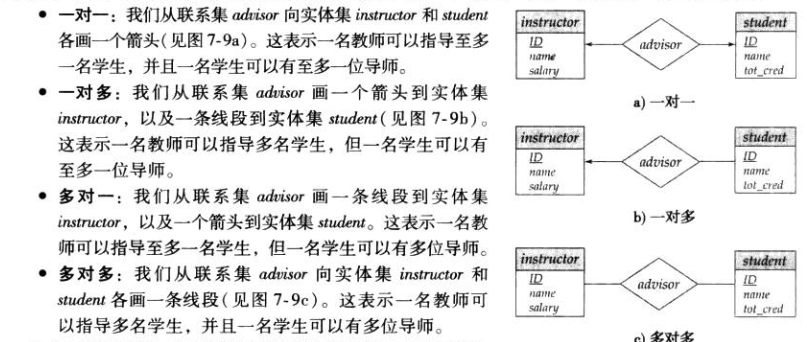
\includegraphics[width=\linewidth]{fig/mapping_radix.png}
\end{figure}
\end{definition}
也可以采用更为复杂的映射基数$l..h$的形式表示,其中$l$表示最小映射基数,$h$为最大映射基数。
最小值为$1$代表这个实体集在该联系集中全部参与,最大值为$1$表示这个实体至多参与一个联系,最大值为$*$则没有限制。

\begin{definition}[角色]
联系集产生自环,如course有前置课程prereq\_id
\end{definition}
\begin{definition}[强弱实体集]
没有足够属性形成主码的实体集称为弱实体集,有主码的实体集则称为强实体集。
弱实体集必须与另一个称作标识(identifying)或\textbf{属主(owner)实体集}的实体集关联才有意义。
弱实体集的\textbf{分辨符}(discriminator)/部分码是使得能够区分弱实体集中实体的方法,用虚下划线标明。
\end{definition}

比如section实体由课程编号、学期、学年及开课编号唯一标识。
假定在实体集section和course之间创建了联系集sec\_course,由于section中已有属性course\_id,故在联系集中存在冗余,要将course\_id删除,但这会导致section没有主码。
因而将联系sec\_course视为特殊的联系,它给唯一标识section实体提供额外信息,即course\_id。

E-R图,菱形代表联系,双横线代表全部参与,双框代表弱实体集。
\begin{figure}[H]
\centering
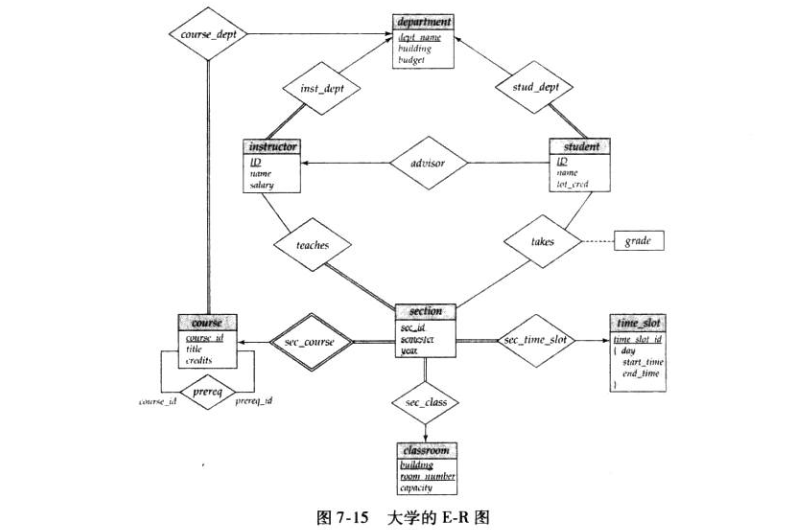
\includegraphics[width=0.6\linewidth]{fig/university_E-R.png}
\end{figure}
\begin{figure}[H]
\centering
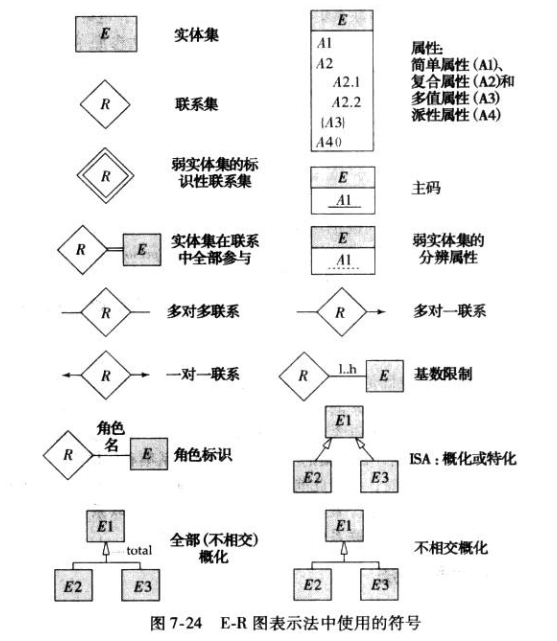
\includegraphics[width=0.5\linewidth]{fig/E-R-figure.png}
\end{figure}

一个常见的错误是将一个实体集的主码作为另一个实体集的属性(关系被隐藏了),而不是使用联系。

\subsection{转化为关系模式}
\begin{itemize}
	\item 简单属性强实体集直接转关系模式,如
	\[student(\underline{ID},name,tot\_cred)\]
	\item 复杂属性强实体集展平后转关系模式,如名字含first\_name和last\_name,那就一起放入关系模式
	\item 弱实体集由\textemph{其依赖的强实体集主码与自身}组成,主码为\underline{强实体集主码与弱实体集分辨符},且要在关系$A$上建立外码约束
	\item 联系集:\textemph{所有参与该联系的实体集的主码的并集}构成属性集合(弱实体集则要带上其依赖的强实体集主码),依据下列规则选择主码:
	\begin{center}
	\begin{tabular}{|c|c|c|}\hline
		A & B & 主码\\\hline
		多 & 多 & A+B\\\hline
		多 & 一 & A\\\hline
		一 & 多 & B\\\hline
		一 & 一 & A/B\\\hline
	\end{tabular}
	\end{center}
	对于每个与联系集$R$相关的实体集$E_i$,建立关系模式$R$上的外码约束,$R$中来自$E_i$主码属性的那些属性参照表示关系模式$E_i$的主码。
	如大学关系模式中,advisor为多对一联系,则建立关系模式
	\[advisor(\underline{s\_ID},i\_ID)\]
\end{itemize}

通常,连接\textemph{弱实体集与其依赖的强实体集的联系集的模式是冗余的},在基于E-R图的关系数据库设计中不必给出。

当出现以下两种情况时,需要对关系模式进行合并:
\begin{itemize}
	\item 实体集$A$到实体集$B$是一个\textemph{多对一}的联系集$AB$,且$A$的\textemph{参与是全部的},则将$A$和$AB$合并,如inst\_dept可以和instructor合并为
	\[instructor(\underline{ID},name,dept\_name,salary)\]
	合并后的主码是$A$的主码。
	\item 一对一则联系集可以跟参与联系的任一个实体集模式进行合并
\end{itemize}

\subsection{扩展的E-R属性}
\begin{definition}[特化和泛化]
在实体集内部进行分组的过程称为特化(specialization),如将实体集person划分为employee和student。
概化(generalization)则是自底向上的反过程。
高层与低层实体集也可被分别称为超类和子类,同样有继承(inheritance)的特性。
如果一个实体集作为低层实体集参与到多个联系中,则称这个实体集具有多继承,且产生的结构称为格(lattice)。
\end{definition}

\begin{definition}[聚集]
聚集是一种抽象,其中联系集和跟它们相关的实体集一起被看作高层实体集,并且可以参与联系。
\end{definition}
% !TEX root = main.tex

\section{关系数据库设计} % Chap 8
好的关系设计的特点:\textbf{避免不必要冗余、无损分解、保持依赖}。

\subsection{范式理论}
定义属性集$\alpha$,关系模式为$r(R)$。
关系模式是一个属性集,但不是所有属性集都是模式。
超码则用$K$来表示。
\begin{definition}[超码]
$R$的子集$K$是$r(R)$的超码的条件是:在关系$r(R)$的任意合法实例中,对于$r$实例中的元组对$t_1$和$t_2$总满足,若$t_1\ne t_2$,则$t_1[K]\ne t_2[K]$,即$K$唯一标识一条元组。(而\textemph{函数依赖则是唯一标识某些属性})
\end{definition}

设计需要满足一定的范式(normal form),核心目的是\textcolor{red}{减少冗余}:
% https://www.geeksforgeeks.org/normal-forms-in-dbms/
\begin{itemize}
	\item \textbf{第一范式(1NF)}:全部属性都是\textemph{单值属性}(原子性)

	\item \textbf{第二范式(2NF)}:关系模式$R\in 1NF$,且每一个\textemph{非主属性\textbf{完全依赖}于$R$的主码},而不是只依赖于其中一部分属性(即其中一部分属性的值即可确定该属性的值,部分依赖)
	\begin{example}
	一个学生-课程关系模式如下:
	\begin{center}
	\begin{tabular}{|c|c|c|}\hline
		Stud\_No & Course\_No & Course\_Fee\\\hline
		1 & C1 & 1000\\
		2 & C2 & 1500\\
		1 & C4 & 2000\\
		4 & C3 & 1000\\
		4 & C1 & 1000\\
		2 & C5 & 2000\\\hline
	\end{tabular}
	\end{center}
	如此例中Stud\_No和Course\_No是主码,但是实际上只由Course\_No就已经可以决定Course\_Fee了,因此这个例子不满足2NF。
	\end{example}

	\item \textbf{第三范式(3NF)}:关系模式$R\in 2NF$,且对于$F^+$中所有形如$\alpha\to\beta$的函数依赖,至少下列一项成立
	\begin{itemize}
		\item $\alpha\to\beta$是一个平凡的函数依赖
		\item $\alpha$是$R$的一个超码
		\item \textemph{$\beta-\alpha$}中的每个属性$A$都含于$R$的一个候选码中\footnote{并不要求单个候选码必须包含$\beta-\alpha$所有属性,$\beta-\alpha$每个属性可能含于不同候选码中。}
	\end{itemize}
	(非主属性依赖于主码但不能通过另一非主属性进行依赖,即\textemph{不存在传递依赖})
	\begin{example}
	一个学生-国家关系模式如下:
	\begin{center}
	\begin{tabular}{ccccc}\hline
	Stud No & Stud Name & Stud State & Stud Country & Stud Age\\\hline
	1 & Alice & s1 & c & 18\\
	2 & Alice & s2 & c & 19\\
	3 & Bob & s2 & c & 21\\\hline
	\end{tabular}
	\end{center}
	有传递依赖Stud No$\to$Stud State$\to$Stud Country,因此不满足3NF。
	\end{example}

	\item \textbf{巴斯-科德/BC范式(Boyce-Codd NF, 3.5NF)}:关系模式$R\in 3NF$,对于$F^+$中所有形如$\alpha\to\beta$的函数依赖,至少有以下一项成立:
	\begin{itemize}
		\item $\alpha\to\beta$是平凡的函数依赖(即$\beta\subset\alpha$)
		\item $\alpha$是模式$R$的一个\textemph{超码}
	\end{itemize}
\end{itemize}

\subsection{函数依赖}
\begin{definition}[函数依赖(functional dependency)]
设$R$为关系模式,$\alpha\subset R,\beta\subset R$,函数依赖$\alpha\to\beta$在$R$上满足,当且仅当对于任意合法的关系$r(R)$,任何两个关于$r$的数对$t_1$和$t_2$,如果满足属性$\alpha$,那么它们也满足属性$\beta$,即
\[t_1[\alpha]=t_2[\alpha]\implies t_1[\beta]=t_2[\beta]\]
实际上就是\textemph{函数单射}的概念,属性$\alpha$可以\textemph{唯一确定}属性$\beta$的值。
若函数依赖$K\to R$在$r(R)$上成立(注意这里$R$相当于全部属性,或者写成$K\to (R-K)$),则$K$是$r(R)$的一个\textemph{超码}。
\end{definition}
\begin{example}
考虑下例$r(A,B)$的关系
\begin{center}
\begin{tabular}{|c|c|}\hline
A & B\\\hline
1 & 4\\\hline
1 & 5\\\hline
3 & 7\\\hline
\end{tabular}
\end{center}
关系$A\to B$不成立,但关系$B\to A$成立。
\end{example}

\begin{definition}[平凡]
在所有关系中都满足的函数依赖则是平凡的函数依赖,比如$A\to A$。
一般地,若$\beta\subset\alpha$,则$\alpha\to\beta$的函数依赖是平凡的。
\end{definition}

\subsubsection{闭包}
\begin{definition}[逻辑蕴含与闭包]
若关系模式$r(R)$的每一个满足$F$的实例也满足$f$,则$R$上的函数依赖$f$被$r$上的函数依赖集$F$逻辑蕴含。
$F$的闭包是被$F$逻辑蕴含的所有函数依赖的集合,记作$F^+$。
设$\alpha$为属性集,将函数依赖集$F$下被$\alpha$函数确定的所有属性的集合称为$F$下$\alpha$的闭包。
\end{definition}

\begin{theorem}[逻辑蕴含公理]
下面的前三条为最基本的公理(Armstrong),可以找出给定$F$的所有$F^+$
\begin{itemize}
	\item \textbf{自反律}(reflexivity):若$\alpha$为一属性集且$\beta\subset\alpha$,则$\alpha\to\beta$
	\item \textbf{增补律}(augmentation):若$\alpha\to\beta$成立且$\gamma$为一属性集,则$\gamma\alpha\to\gamma\beta$成立
	\item \textbf{传递律}(transitivity):若$\alpha\to\beta$和$\beta\to\gamma$成立,则$\alpha\to\gamma$成立
	\item 合并律(union):若$\alpha\to\beta$和$\alpha\to\gamma$成立,则$\alpha\to\beta\gamma$成立
	\item 分解律(decomposition):若$\alpha\to\beta\gamma$成立,则$\alpha\to\beta$和$\alpha\to\gamma$成立
	\item 伪传递律(pseudotransitivity):若$\alpha\to\beta$和$\gamma\beta\to\delta$成立,则$\alpha\gamma\to\delta$成立
\end{itemize}
\end{theorem}

\begin{algorithm}
\caption{计算$F^+$}
\begin{algorithmic}[1]
\State $F^+:=F$
\Repeat
\State 对$F^+$的函数依赖应用自反律、增补律和传递律,将结果加入$F^+$
\Until{result 不变}
\end{algorithmic}
\end{algorithm}
由于包含$n$个元素的集合有$2^n$个子集,因此总共有$2^{2n}$个可能的函数依赖在$F^+$中。

\begin{algorithm}[H]
\caption{计算$F$下属性$\alpha$的闭包$\alpha^+$}
\begin{algorithmic}[1]
\State result$:=\alpha$
\Repeat
\For{每一个函数依赖$\beta\to\gamma\in F$}
\State 若$\beta\subset$ result,则result $:=$ result $\cup$ $\gamma$
\EndFor
\Until{result 不变}
\end{algorithmic}
\end{algorithm}

属性闭包算法有多种用途:
\begin{itemize}
	\item 用于\textemph{判断$\alpha$是否为超码},计算$\alpha^+$,检查$\alpha^+$是否包含$R$中所有属性
	\item 通过检查是否$\beta\subset\alpha^+$,我们可以检查$\alpha\to\beta$是否成立(即是否属于$F^+$),也就是用属性闭包计算$\alpha^+$,看是否包含$\beta$
	\item 另一种计算$F^+$的方法:$\forall\gamma\subset R$,找出$\gamma^+$;$\forall S\subset\gamma^+$,输出函数依赖$\gamma\to S$
\end{itemize}

\begin{example}
为求解候选码,要将属性集的所有子集尝试一遍,每个都求属性闭包,看是否覆盖所有属性,如果是则为超码,进一步选择最小的集合作为候选码。
比如ABC,则尝试
\[A,B,C,AB,AC,BC,ABC\]
算这些属性集的属性闭包看是否全覆盖。
\end{example}

\subsubsection{正则覆盖}
\begin{definition}[无关(extraneous)]
如果去除函数依赖中的一个属性不改变该函数依赖集的闭包,则称该属性是无关的,即\textemph{去掉该属性依然可以推得其函数依赖成立},形式化定义即
\begin{itemize}
	\item 若$A\in\alpha$且$F$逻辑蕴含$(F-\{\alpha\to\beta\})\cup\{\textcolor{blue}{(\alpha-A)\to\beta}\}$,则属性$A$在$\alpha$中无关
	\item 若$A\in\beta$且$(F-\{\alpha\to\beta\})\cup\{\textcolor{blue}{\alpha\to(\beta-A)}\}$逻辑蕴含$F$,则属性$A$在$\beta$中无关
\end{itemize}
\end{definition}

检验属性$A$是否无关的方法如下:
\begin{itemize}
	\item 若$A\in\alpha$,为检验$A$是否无关,令$\gamma=\alpha-\{A\}$,检验\textemph{$\gamma\to\beta$}是否可以由$F$推出\\
	计算$F$下的$\gamma^+$,若$\gamma^+$包含$\beta$中所有属性,则$A$在$\alpha$中无关。
	\item 若$A\in\beta$,为检验$A$是否无关,令$F'=(F-\{\alpha\to\beta\})\cup\{\alpha\to(\beta-A)\}$,检验\textemph{$\alpha\to A$}是否能由$F'$推出\\
	计算$F'$下的$\alpha^+$,若$\alpha^+$包含$A$,则$A$在$\beta$中无关。
\end{itemize}

\begin{definition}[正则覆盖(canonical cover)]
$F$的正则覆盖$F_c$是一个依赖集,使得$F_c$和$F$双向逻辑蕴含,且
\begin{itemize}
	\item $F_c$中任何函数依赖都不含无关属性
	\item $F_c$中函数依赖的左半部都是唯一的,即不存在$\alpha_1\to\beta_1$和$\alpha_2\to\beta_2$满足$\alpha_1=\alpha_2$
\end{itemize}
\end{definition}
\begin{algorithm}
\caption{计算正则覆盖}
\begin{algorithmic}[1]
\State $F_c=F$
\Repeat
\State 用\textemph{合并律}将$F_c$中$\alpha_1\to\beta_1$和$\alpha_1\to\beta_2$替换为$\alpha_1\to\beta_1\beta_2$
\State 对$F_c$每一个函数依赖\textemph{移除无关属性}
\Until{$F_c$不变}
\end{algorithmic}
\end{algorithm}

\subsubsection{无损分解与保持依赖的分解}
\begin{definition}[无损分解]
令$R_1$和$R_2$为$R$的分解,用$r_1(R_1)$和$r_2(R_2)$代替$r(R)$没有信息损失,则为无损(lossless)分解。
\[\Pi_{R_1}(r)\Join\Pi_{R_2}(r)=r\]
否则为有损分解。
\end{definition}
考虑employee模式的分解
\[\begin{array}{l}
employee1 (ID,name)\\
employee2 (name,street,city,salary)
\end{array}\]
当两个员工有相同名字时,丢失员工标识与地址工资相关联信息,故分解是有损的。

\begin{theorem}
若$R_1$和$R_2$是$R$的无损分解,则下列函数依赖至少有一个属于$F^+$
\begin{itemize}
	\item $R_1\cap R_2\to R_1$
	\item $R_1\cap R_2\to R_2$
\end{itemize}
即\textemph{$R_1\cap R_2$是$R_1$或$R_2$的超码}。
\end{theorem}

\begin{definition}[保持依赖的分解]
$F$是模式$R$上一个函数依赖集,$R_i$为$R$的一个分解,$F$在$R_i$上限定(restriction)是$F^+$中所有\textbf{只包含}$R_i$中属性的函数依赖的集合$F_i$。
令$F'=\bigcup_i F_i$,具有$F'^+=F^+$的分解为保持依赖的分解。
\end{definition}

两种避免计算$F^+$验证保持依赖的方法:
\begin{itemize}
	\item 若$F$中每一个函数依赖都可以在分解得到的某一个关系上验证,那么这个分解就是保持依赖的。(注意这只是必要不充分条件。)
	\item 对$F$中每一个$\alpha\to\beta$应用
\begin{center}
\begin{algorithmic}[1]
\State $result:=a$
\Repeat
\For{each $R_i$}
\State $t=(result\cap R_i)^+\cap R_i$
\State $result :=result\cup t$
\EndFor
\Until{$result$没有变化}
\end{algorithmic}
\end{center}
这里的属性闭包是$F$下的,若$result$包含$\beta$所有属性,则$\alpha\to\beta$保持。
分解是保持依赖的当且仅当上述过程中$F$所有依赖都保持。
\end{itemize}

\subsection{分解算法}
\subsubsection{BCNF分解}
简化判定方法:
\begin{itemize}
	\item 检查非平凡函数依赖$\alpha\to\beta$,计算$\alpha^+$,验证它是否包含$R$中所有属性,即验证它是否为$R$的超码;不需检查$F^+$中所有函数依赖(但分解后就不能这么做了)
	\item 对$R_i$中属性每个子集$\alpha$,确保$F$下$\alpha^+$要么不含$R_i-\alpha$的任何属性,要么包含$R_i$所有属性。若$R_i$上有某个属性集$\alpha$违反条件,即下述函数依赖会出现在$F^+$中,说明违反BCNF
	\[\alpha\to(\alpha^+-\alpha)\cap R_i\]
\end{itemize}
\begin{algorithm}
\caption{BCNF分解}
\begin{algorithmic}[1]
\State 初始化result $:=\{R\}$
\State 计算$F^+$
\State 若result中存在模式$R_i$不属于BCNF,$\alpha\to\beta$为$R_i$上成立的非平凡函数依赖,满足$\alpha\to R_i$不属于$F^+$,且$\alpha\cap\beta=\varnothing$,则将其分解为$(R_i-\beta)$和$(\alpha,\beta)$
\end{algorithmic}
\end{algorithm}

不依据伪码进行分解则直接将不满足BCNF的替换为\textemph{$R-(\beta-\alpha)$和$\alpha\cup\beta$}即可。

\subsubsection{3NF分解}
\begin{algorithm}
\caption{3NF分解}
\begin{algorithmic}[1]
\State 令$F_c$为$F$的\textemph{正则覆盖}
\State 对于每一个$F_c$中的函数依赖$\alpha\to\beta$,\textemph{$R_i=\alpha\beta$}
\State 若$R_i$都不包含$R$的候选码,则新增$R_{i+1}$为$R$的\textemph{候选码}
\State 若$R_j\in R_k$,则删除$R_j$,直至不再有可删除的$R_j$
\end{algorithmic}
\end{algorithm}

\subsection{多值依赖}
函数依赖规定了某些元组不能出现在关系中。
如果$A\to B$,则不能有两个元组在$A$上的值相同,而在$B$上值不同。
多值依赖不排除某些元组的存在,而要求某种形式的其他元组存在于关系中。
函数依赖称为相等产生(equality-generating)依赖,多值依赖称为元组产生依赖。
\begin{definition}[多值依赖(multivalued dependency)]
设$R$为关系模式,$\alpha\subset R,\beta\subset R$,多值依赖在$R$上满足$\alpha\to\to\beta$,% \twoheadrightarrow
当且仅当对于所有数对$t_1$和$t_2$,使得$t_1[\alpha]=t_2[\alpha]$,都存在数对$t_3$和$t_4$使得
\[\begin{aligned}
\displaystyle t_{1}[\alpha ]&= t_{2}[\alpha ]=t_{3}[\alpha ]=t_{4}[\alpha ]\\
\displaystyle t_{3}[\beta ]&= t_{1}[\beta ]\\
\displaystyle t_{3}[R-\beta ]&= t_{2}[R-\beta ]\\
\displaystyle t_{4}[\beta ]&= t_{2}[\beta ]\\
\displaystyle t_{4}[R-\beta ]&= t_{1}[R-\beta ]
\end{aligned}\]
简而言之,若${\displaystyle (a,b,c)}$和${\displaystyle (a,d,e)}$在$R$中,则${\displaystyle (a,b,e)}$和${\displaystyle (a,d,c)}$在$R$中。
即两个属性互相独立,但是都依赖于第三个属性。
\begin{center}
\begin{tikzcd}
 & b\arrow[rdd]\arrow[r] & c\\
a\arrow[ru]\arrow[rd] & &\\
 & d\arrow[ruu]\arrow[r] & e
\end{tikzcd}
\end{center}
典型例子是$(\text{课程},\text{课本},\text{老师})$,一门课有两本课本,两个老师,课本和老师之间不存在函数依赖,但都依赖于课程。
\end{definition}

令$D$表示函数依赖和多值依赖的集合,则$D^+$是由$D$逻辑蕴含的所有函数依赖和多值依赖的集合。
对于多值依赖有以下规则
\begin{itemize}
	\item 每个函数依赖都是一个多值依赖,即若$\alpha\to\beta$,则$\alpha\to\to\beta$
	\item 若$\alpha\to\to\beta$,则$\alpha\to\to R-\alpha-\beta$
\end{itemize}

第四范式(4NF):函数依赖和多值依赖集为$D$的关系模式$r(R)$属于第四范式的条件是对$D^+$中所有形如$\alpha\to\to\beta$的多值依赖$\alpha,\beta\subset R$,至少有以下之一成立:
\begin{itemize}
	\item $\alpha\to\to\beta$是一个平凡的多值依赖
	\item $\alpha$是$R$的一个超码(这里已经蕴含了$4NF\in BCNF$)
\end{itemize}
% !TEX root = main.tex

\section{索引与散列} % Chap 11
\subsection{基本概念}
通常索引文件包含记录/索引项,要比原文件小很多
\begin{center}
\begin{tabular}{|c|c|}\hline
search-key & pointer\\\hline
\end{tabular}
\end{center}

两种基本的索引类型:顺序(ordered)索引、散列(hash)索引

\subsection{顺序索引}
\begin{definition}[聚集索引]
在顺序索引中,包含记录的文件按照某个\textbf{搜索码}指定顺序排序,则该搜索码对应的索引称为聚集索引(clustering index),也被称为主索引(primary)。
但注意并\textbf{不是建立在主码上的索引}。
若搜索码指定的顺序与文件中记录的物理顺序不同,则称为非聚集索引(secondary)。
\end{definition}
\begin{definition}[稠密/稀疏索引]
对于每个搜索码都出现索引记录的称为稠密索引,只包含特定搜索码值的称为稀疏索引。
非聚集索引一定是稠密的。
\end{definition}

稀疏索引查找方法即找到最大搜索码键值小于$K$的,然后继续往下搜索。
\begin{figure}[H]
\centering
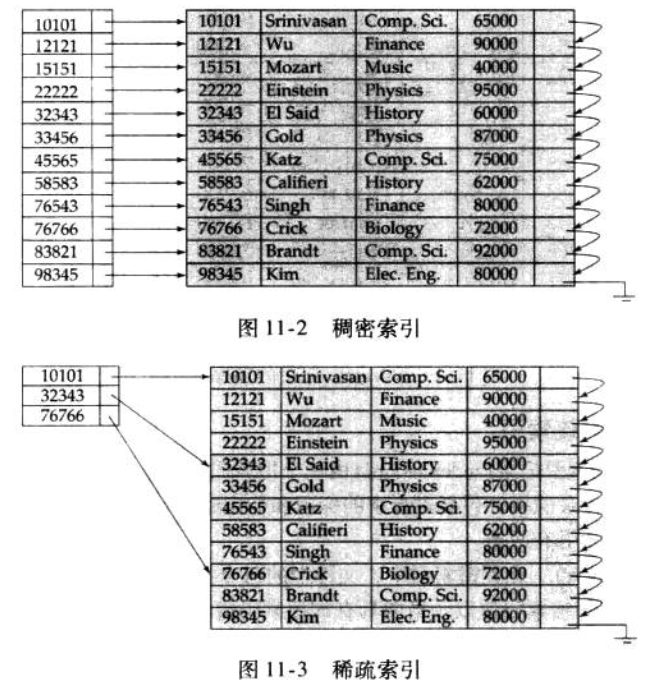
\includegraphics[width=0.6\linewidth]{fig/dense_sparse_indexing.png}
\end{figure}

通过建造多级稀疏索引,来减少访问时间。
\begin{figure}[H]
\centering
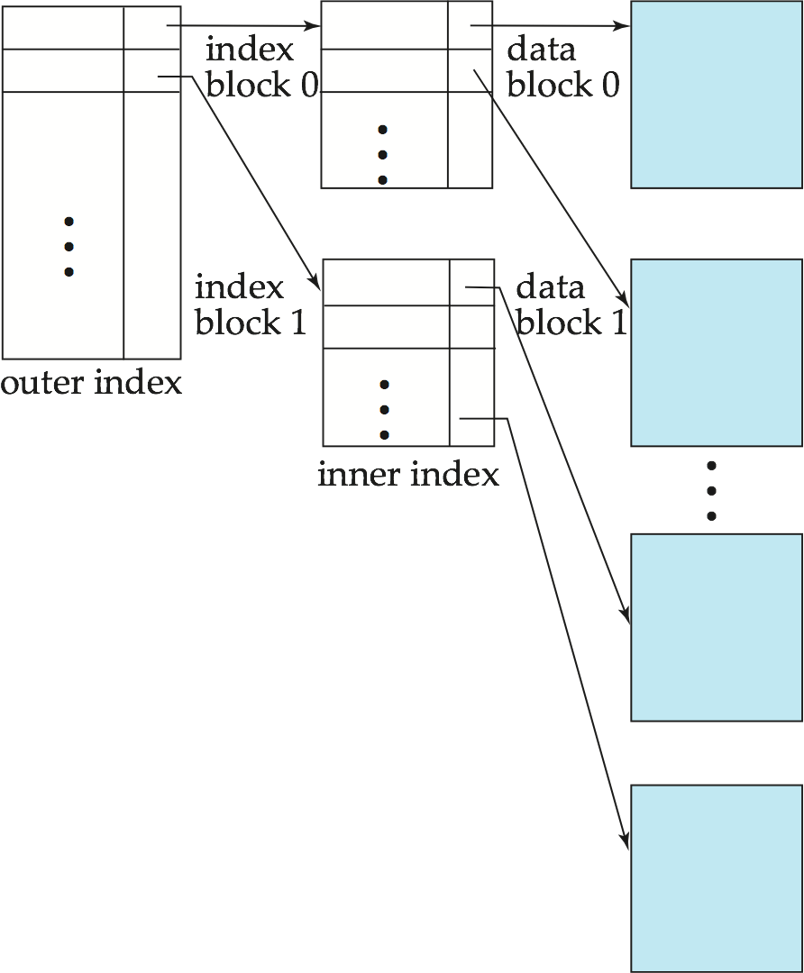
\includegraphics[width=0.5\linewidth]{fig/multilevel-index.png}
\end{figure}

索引更新操作:
\begin{itemize}
	\item 删除:稠密连同搜索码直接删,稀疏判大小
	\item 插入:同上直接插
\end{itemize}

\subsection{B+树索引}
当文件大起来时上述索引变得很慢,周期性更新整个文件非常麻烦,因此有B+树自动管理小的局部插入删除。

\subsubsection{基本性质}
B+树索引采用平衡树结构,树根到树叶的每条路径长度相同。
$n$-阶B树满足以下性质:
\begin{itemize}
	\item 所有叶子结点都必须在同一层
	\item 除了根结点外的\textbf{非叶子节点}都至少有$\lceil n/2\rceil$个孩子,至多$n$个孩子
	\item 叶子结点至少有\textcolor{red}{$\lceil (n-1)/2\rceil$}个关键字,最多$n-1$个关键字
	\item 特殊情况:
	\begin{itemize}
		\item 根节点不是叶子,则至少有$2$个孩子
		\item 根节点是叶子,则可以有$[0,n-1]$个值
	\end{itemize}
	\item 每个结点有$n$个指针,$n-1$个键值/搜索码\textbf{升序排序}(通常是严格不等式)
	\begin{center}
	\begin{tabular}{|c|c|c|c|c|c|c|}\hline
	$P_1$ & $K_1$ & $P_2$ & $\cdots$ & $P_{n-1}$ & $K_{n-1}$ & $P_n$\\\hline
	\end{tabular}
	\end{center}
	\item 左侧的叶子结点的搜索码值一定都小于\textbf{等于}右侧的叶子结点的搜索码值
	\item 指针与其\textbf{后面}的键值为一组,即$P_i$指向搜索码值为$K_i$的记录(叶子结点),或$P_i$指向$[K_{i-1},K_i)$(非叶子节点,注意右侧不包含);$P_n$指向下一个叶子节点
\end{itemize}

而B+树则是将所有关键字存储在叶子结点,其他结点作为索引,并且为每个叶子结点增加一个链指针。
\begin{figure}[H]
\centering
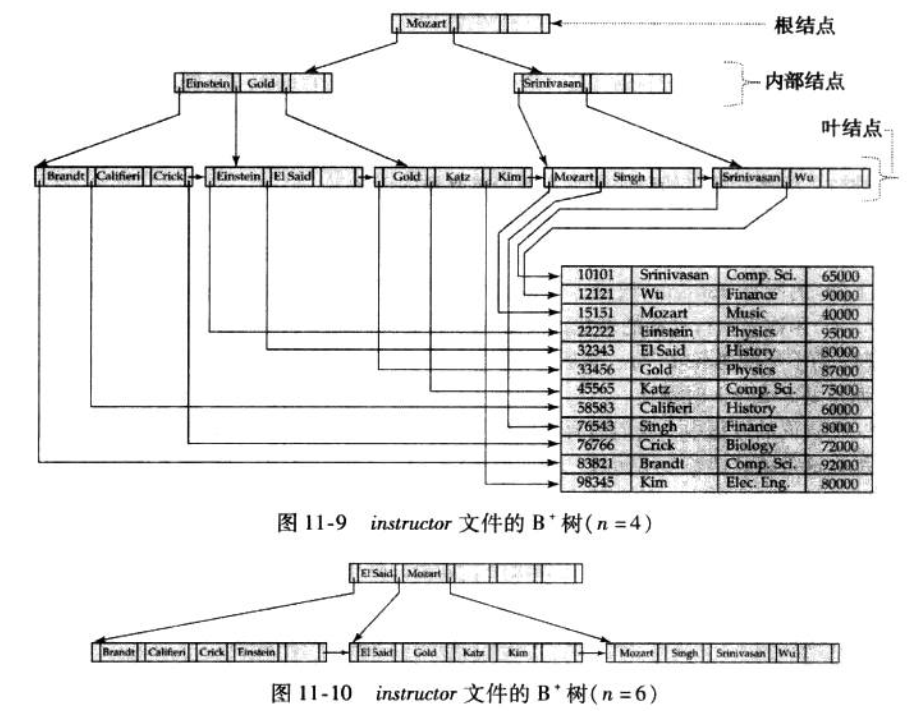
\includegraphics[width=0.6\linewidth]{fig/bp-tree.png}
\end{figure}

根节点下至少有$2\lceil n/2\rceil$个键值,下一层至少$2\lceil n/2\rceil^2$个,以此类推;
若记录中有$K$个搜索码值,则B+树树高不会高过$\lceil\log_{\lceil n/2\rceil}(K)\rceil$。

% 重复?

\subsubsection{插入}
\begin{itemize}
	\item 搜索码值已经存在于叶子结点:直接加记录
	\item 搜索码值没有出现,添加记录到主文件,插入到叶子节点;如果没有位置,需要进行分裂
	\begin{itemize}
		\item 将这$n$个$(\text{搜索码值},\text{指针})$进行排序,取前$\lceil n/2\rceil$个在原来节点,其余在新节点
		\item 令新节点为$p$,$k$为$p$中的最小值,则插入$(k,p)$到父亲中,$p$为$k$的后续指针
		\item 若父亲满了,则继续分裂并传播
	\end{itemize}
\end{itemize}
\begin{figure}[H]
\centering
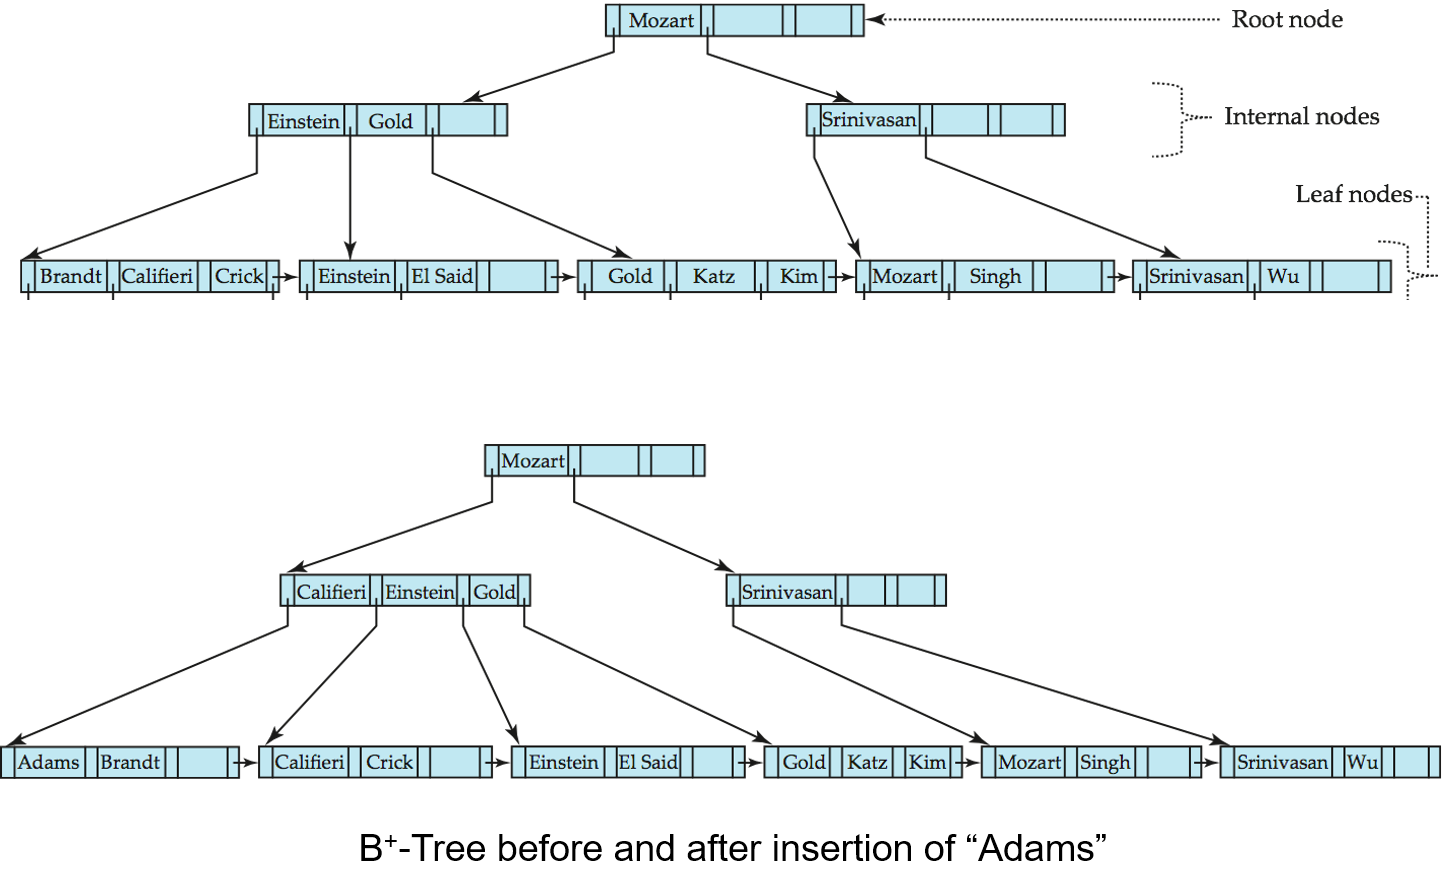
\includegraphics[width=0.8\linewidth]{fig/bp-tree_insertion.png}
\end{figure}

\subsubsection{删除}
\begin{itemize}
	\item 直接移除
	\item 如果删除导致下溢(underfull),则需要合并兄弟
	\begin{itemize}
		\item 若\textemph{兄弟节点}未满,则与兄弟节点合并(注意不是同层都是兄弟)
		\item 删除$(K_{i-1},P_i)$,其中$P_i$是指向删除结点的指针,递归这个过程
	\end{itemize}
	\item 如果合并没法合到一个节点,则需要\textbf{重分配}(redistribute)指针使得两个节点都含有多于最小键值数目的项。
	将左侧分配到右侧,并重新分配指针
\end{itemize}
\begin{figure}[H]
\centering
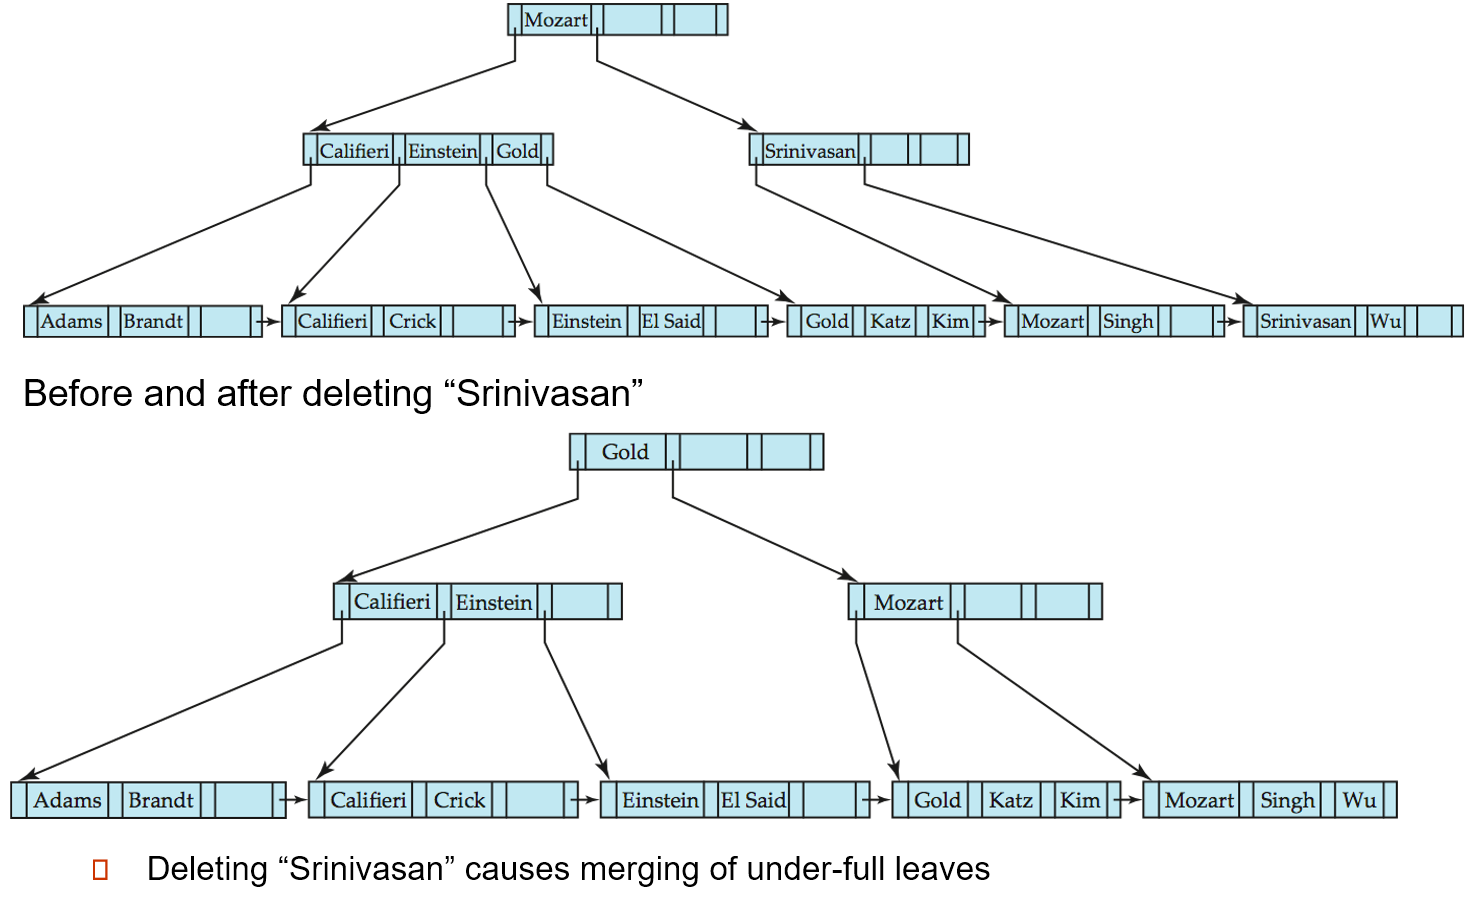
\includegraphics[width=0.8\linewidth]{fig/bp-tree_deletion.png}
\end{figure}
\begin{figure}[H]
\centering
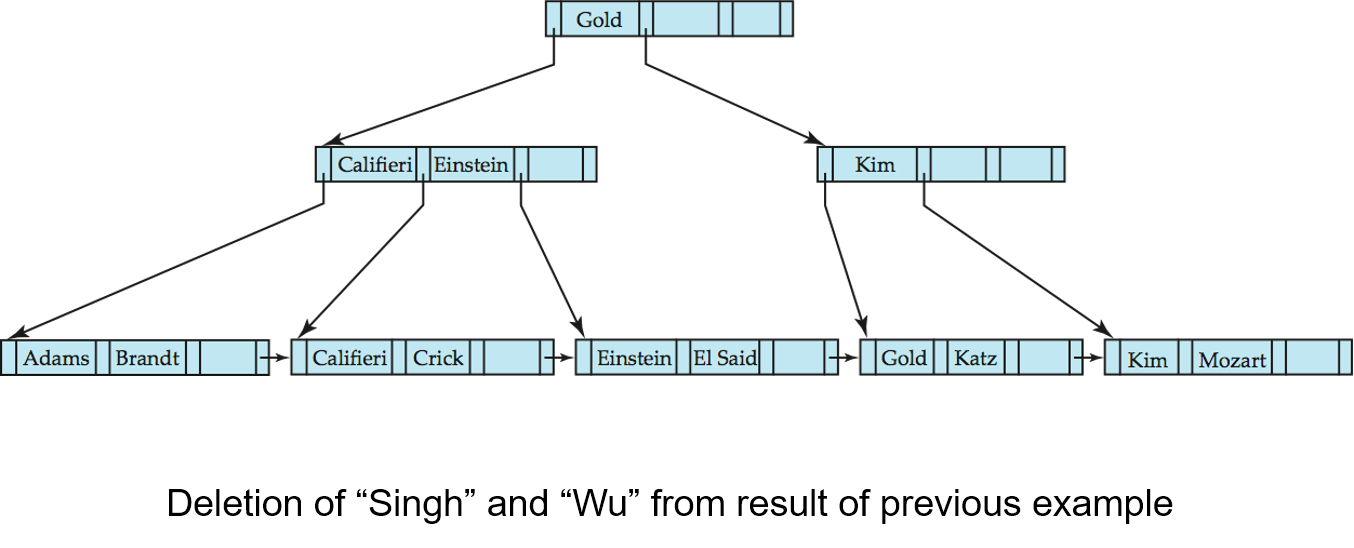
\includegraphics[width=0.8\linewidth]{fig/bp-tree_deletion2.png}
\end{figure}
\begin{figure}[H]
\centering
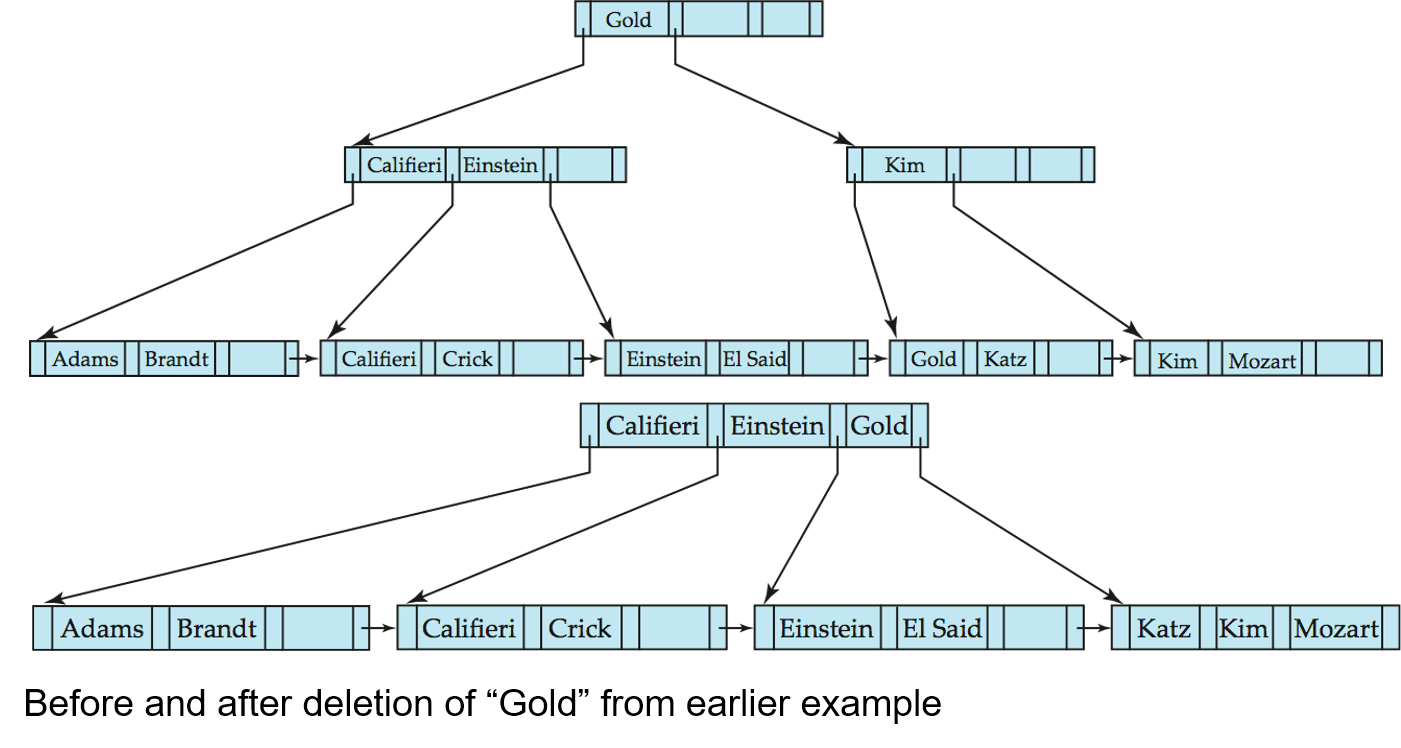
\includegraphics[width=0.8\linewidth]{fig/bp-tree_deletion3.png}
\end{figure}

\subsubsection{其他事项}
\begin{itemize}
	\item 前缀压缩:比如``abcde''和``abds''可以通过``ab''进行区分
	\item 多码索引:构成元组进行索引
\end{itemize}

\subsubsection{B+树文件组织}
\begin{figure}[H]
\centering
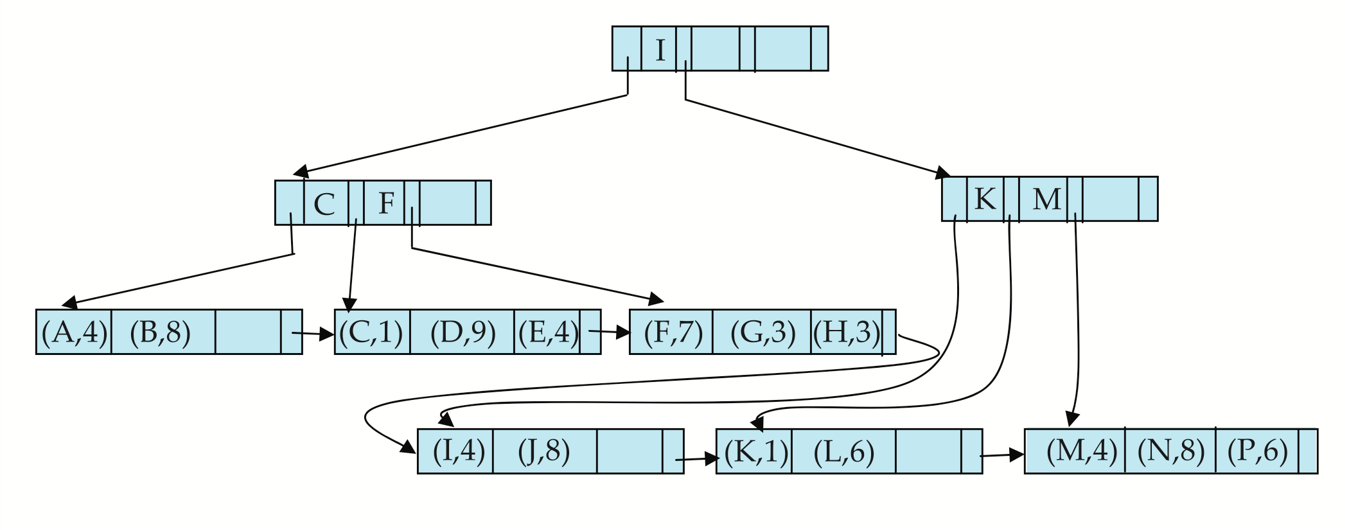
\includegraphics[width=0.8\linewidth]{fig/bp-tree_file_organization.png}
\end{figure}

\subsubsection{B树}
\begin{figure}[H]
\centering
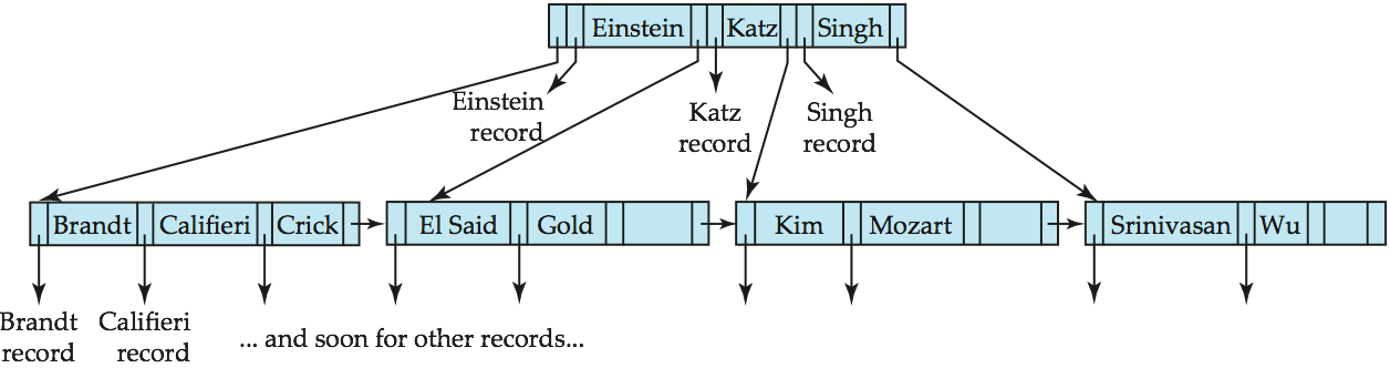
\includegraphics[width=0.8\linewidth]{fig/b-tree.png}
\end{figure}

\subsection{静态散列}
散列(hash)函数应该满足:
\begin{itemize}
	\item 分布均匀:为每个桶分配同样数量的搜索码值
	\item 分布随机:不应与搜索码的任何外部可见排序相关
\end{itemize}

两种散列结构:
\begin{itemize}
	\item 闭散列:一个桶的溢出桶都用链表链接在该桶后面形成溢出链(overflow chaining)
	\item 开散列:线性探查法(probing)插入到下一个有空间的桶
\end{itemize}

下例的散列函数为ID各位数字之和对8取模
\begin{figure}[H]
\centering
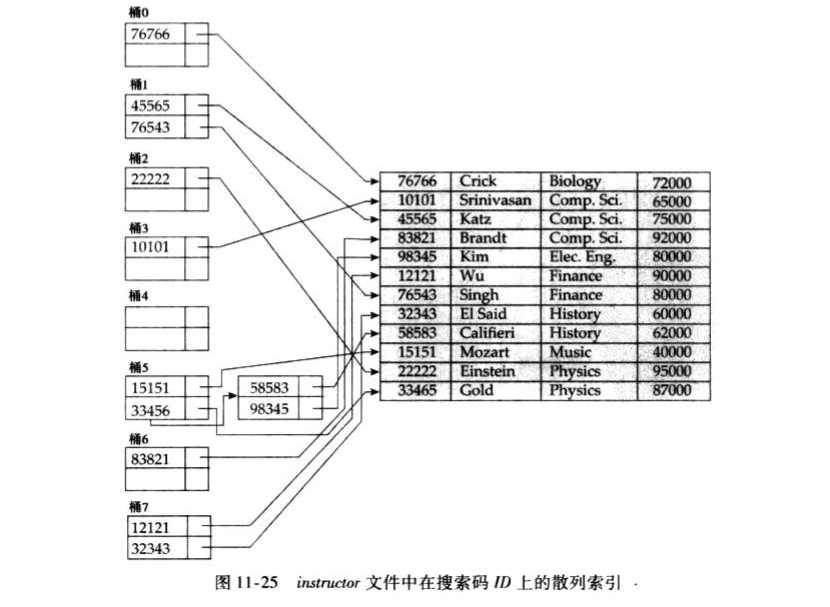
\includegraphics[width=\linewidth]{fig/hash_index.png}
\end{figure}

静态散列问题:
\begin{itemize}
	\item 太小导致后期冲突多性能下降
	\item 太大则大量空间被浪费
\end{itemize}

\subsection{动态散列}
当数据库增大或缩小时,可扩充散列(extendable hashing)可通过桶的分裂或合并来适应数据库大小变化。

通过哈希函数的前$i$位确定索引
\begin{figure}[H]
\centering
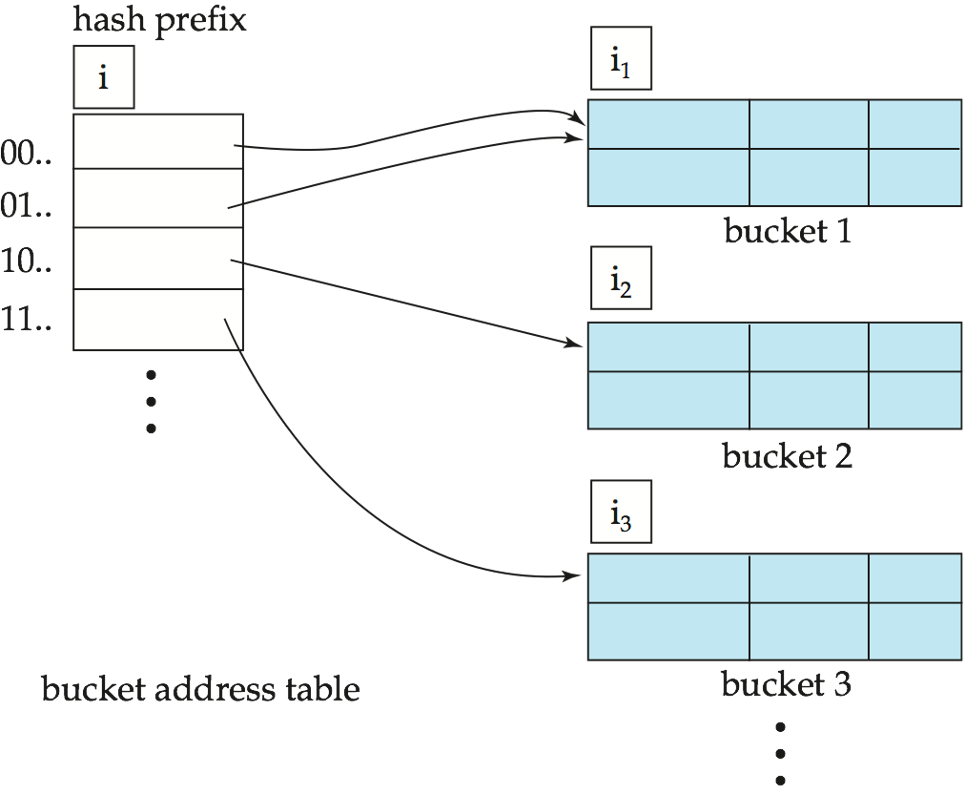
\includegraphics[width=0.6\linewidth]{fig/extendable_hash.png}
\end{figure}
但缺点在于查找涉及一个附加的间接层,系统在访问桶本身之前必须先访问桶地址表。

\subsection{位图索引}
一共是元组个数$n$位,若第$i$个元组的该属性为某特定值,则设为1,否则置0。
\begin{figure}[H]
\centering
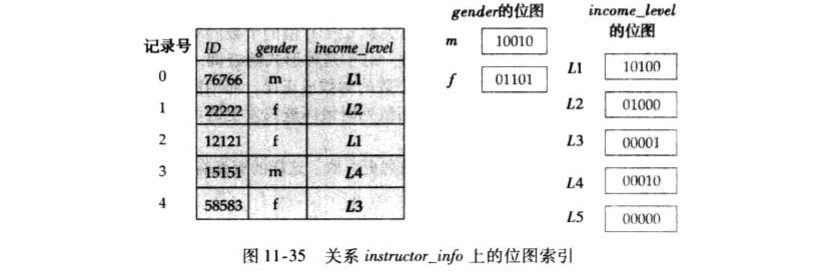
\includegraphics[width=0.9\linewidth]{fig/bitmap.png}
\end{figure}
% !TEX root = main.tex

\section{事务} % Chap 14
\subsection{基本概念}
\begin{definition}[事务(transaction)]
构成单一逻辑工作单元的操作集合称为事务。
即使有故障,数据库系统也必须保证数据库的正确执行——要么执行整个事务,要么属于该事务的操作一个也不执行。
\end{definition}

事务具有以下的基本性质(ACID):
\begin{itemize}
	\item 原子性(Atomicity):要么执行完,要么不执行,不能执行到一半。
	\item 一致性(Consistency):除了基本的数据完整性约束,还有更多的一致性约束。
	\item 隔离性(Isolation):每个事务都察觉不到系统中有其他事务在并发执行,一定是完成一个再进行下一个。
	\item 持久性(Durability):一个事务成功完成对数据库的改变是永久的,即使出现系统故障。
\end{itemize}

事务的基本状态:
\begin{itemize}
	\item 活动的(active):初始状态
	\item 部分提交的(partially commited):最后一条语句执行后
	\item 失败的(failed):执行出错
	\item 中止的(aborted):事务回滚且数据库已恢复到事务开始执行前
	\item 提交的(commited):成功完成
\end{itemize}
\begin{figure}[H]
\centering
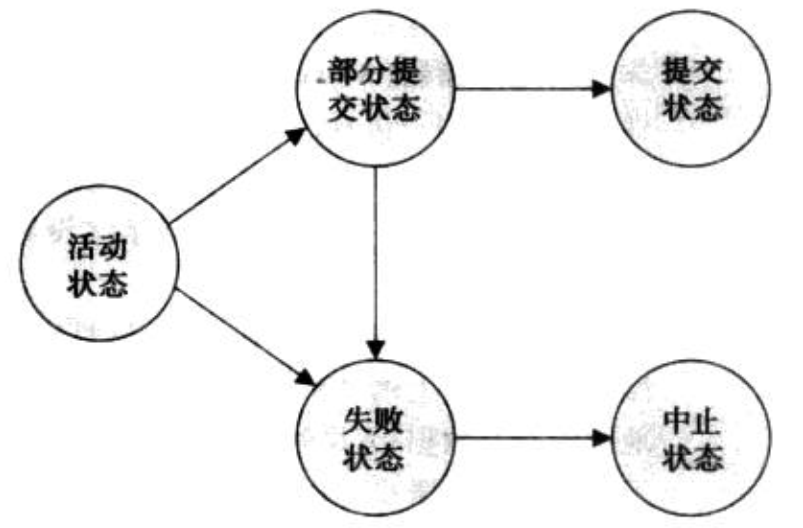
\includegraphics[width=0.5\linewidth]{fig/transaction_state.png}
\end{figure}

\subsection{可串行化}
\begin{definition}[调度]
按照时间顺序执行的一串指令即为调度。
如果事务内的指令都不被打乱,如$<T_1,T_2>$或$<T_2,T_1>$,则为串行调度。
\end{definition}
\begin{definition}[冲突]
当$I$和$J$是不同事务在相同数据项$Q$上的操作,并且其中\textbf{至少有一个}是\verb'write'指令时,则称$I$与$J$是冲突的。
\end{definition}
\begin{definition}[冲突等价(conflict equivalent)]
如果调度$S$可以经过一系列\textbf{非冲突}指令交换转换为$S'$,则称$S$和$S'$是冲突等价的。
若$S'$为串行调度,则$S$为冲突可串行化的(conflict serializable)。
\end{definition}
\begin{figure}[H]
\centering
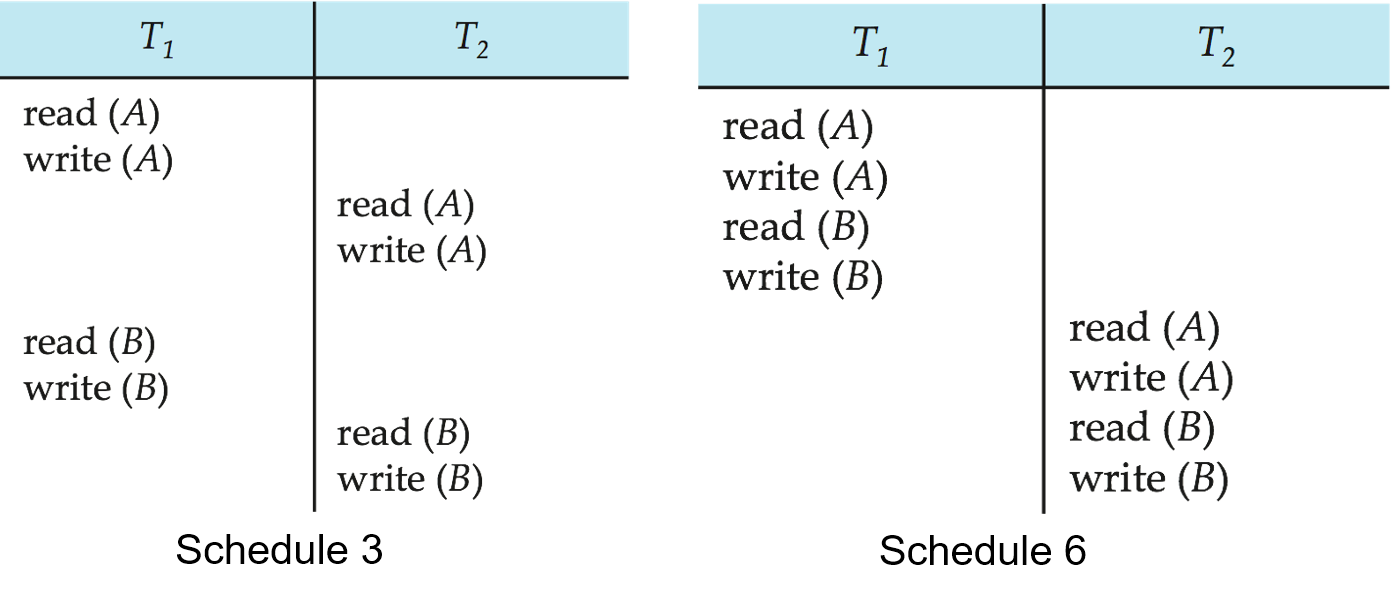
\includegraphics[width=0.8\linewidth]{fig/conflict_serializability.png}
\end{figure}
可以将左侧调度转为右侧,故是冲突可串行的。

可以通过构造一个优先图(precedence graph)来判断是否冲突可串行化。
如果无环(用环检测算法),则冲突可串行化,可以通过\textbf{拓扑排序}(所有父亲执行完才到孩子执行)得到串行化顺序。

\begin{definition}[可恢复调度]
若事务$T_j$读事务$T_i$先前写的数据,则$T_i$的提交必须在$T_j$的提交之前。
\end{definition}

\subsection{隔离性级别}
\begin{itemize}
	\item 可串行化(serializable)
	\item 可重复读(repeatable read)
	\item 已提交读(read committed)
	\item 未提交读(read uncommitted)
\end{itemize}
% !TEX root = main.tex

\section{并发控制} % Chap 15
\subsection{基于锁的协议}
\begin{itemize}
	\item 共享锁(shared):如果事务$T_i$获得了数据项$Q$上的共享型锁(记为$S$),则$T_i$\textbf{可读但不能写}$Q$
	\item 排他锁(exclusive):如果事务$T_i$获得了数据项$Q$上的排他型锁(记为$X$),则$T_i$既\textbf{可读又可写}$Q$
\end{itemize}

若某个事务请求的锁与其他事务持有的锁相容(\textemph{只有共享锁互相相容}),它才可以被授予锁;否则等待所有不相容锁释放。
\begin{table}
\centering
\caption{锁相容性矩阵comp}
\begin{tabular}{|c|c|c|}\hline
 & $S$ & $X$\\\hline
$S$ & true & false\\\hline
$X$ & false & false\\\hline
\end{tabular}
\end{table}

容易发生如下死锁
\begin{figure}[H]
\centering
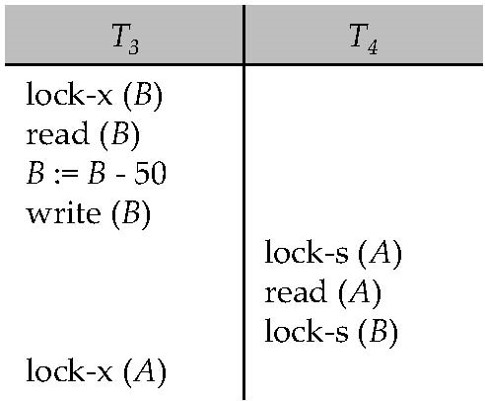
\includegraphics[width=0.3\linewidth]{fig/deadlock.jpg}
\end{figure}

令$\{T_0,\ldots,T_n\}$是参与调度$S$的一个事务集,若存在数据项$Q$,使得$T_i$在$Q$上持有$A$型锁,之后$T_j$在$Q$上持有$B$型锁,且$comp(A,B)=false$,则称在$S$中$T_i$先于$T_j$,记为$T_i\to T_j$,即在任何等价的串行调度中,$T_i$必须出现在$T_j$之前。

避免饿死:当事务$T_i$申请对$Q$加$M$型锁时,授予加锁的条件
\begin{itemize}
	\item 不存在$Q$上持有与$M$型锁相冲突的锁
	\item 不存在等待对数据项$Q$加锁且先于$T_i$申请加锁的事务
\end{itemize}

两阶段封锁协议:可保证冲突可串行化,但不能保证不发生死锁,对于\textbf{每个事务}有以下两个阶段
\begin{enumerate}
	\item 增长(growing)阶段:事务可以获得锁,但不能释放锁(也包括锁的升级,共享$\to$排他)
	\item 缩减(shrinking)阶段:事务可以释放锁,但不能获得新锁(也包括锁的降级,排他$\to$共享)
\end{enumerate}
封锁点为最后加锁的地方。

严格两阶段封锁:所有排他锁要在事务提交后释放,可避免级联回滚。

强两阶段封锁:提交前不能释放任何锁,保证按其提交顺序串行化。

\begin{figure}[H]
\centering
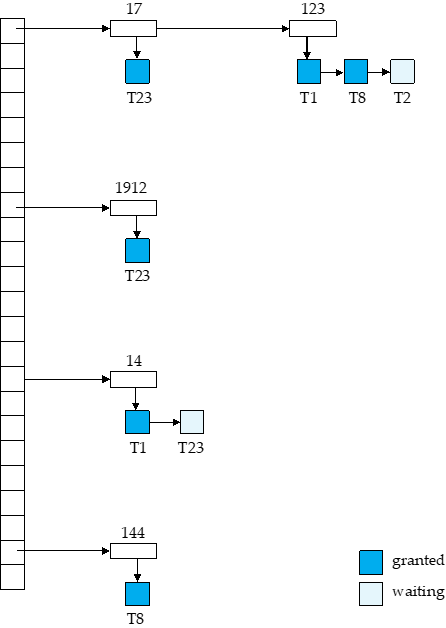
\includegraphics[width=0.4\linewidth]{fig/lock_table.png}
\end{figure}

自动为事务产生适当的加锁、解锁指令:
\begin{itemize}
	\item 事务$T_i$进行$read(Q)$操作时,系统产生一条$lock-S(Q)$指令,该$read(Q)$指令紧跟其后
	\item 事务$T_i$进行$write(Q)$操作时,系统检查$T_i$是否已在$Q$上持有共享锁。
	若有,则系统发出$upgrade(Q)$指令,后接$write(Q)$指令。
	否则系统发出$lock-X(Q)$指令,后接$write(Q)$指令。
	\item 当一个事务提交或中止后,该事务持有的所有锁都被释放。
\end{itemize}

\subsection{基于图的协议}
要求所有数据项集合$D=\{d_1,d_2,\ldots,d_n\}$满足偏序$\to$:如果$d_i\to d_j$,则任何既访问$d_i$又访问$d_j$的事务必须首先访问$d_i$,然后访问$d_j$。
偏序意味着集合$D$可以视为有向无环图,称为数据库图。
\begin{figure}[H]
\centering
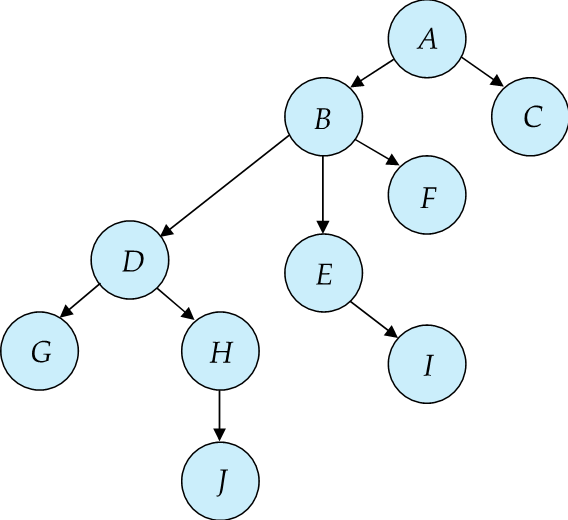
\includegraphics[width=0.4\linewidth]{fig/tree_protocol.png}
\end{figure}

在树形协议中,可用的加锁指令只有lock-X。
每个事务$T_i$对一数据项最多能加一次锁,并且遵从以下规则:
\begin{enumerate}
	\item $T_i$首次加锁可以对任何数据项进行
	\item 此后,$T_i$对数据项$Q$加锁的前提是$T_i$当前持有$Q$的父项上的锁
	\item 对数据项解锁可以随时进行
	\item 数据项被$T_i$加锁并解锁后,$T_i$不能再对该数据项加锁
\end{enumerate}
所有满足树形协议的调度都是冲突可串行化的,且保证不会发生死锁。

但是不满足可恢复性,而且需要给不需要访问的数据也上锁,增加上锁开销,降低并行程度。

\subsection{死锁处理}
\subsubsection{死锁预防}
\begin{itemize}
\item 同时获得所有锁
\begin{itemize}
	\item 每个事务都要在它执行前锁上它所有要用的数据(预声明)
	\item 强加偏序条件(基于图的协议)
\end{itemize}

\item 抢占与事务回滚
\begin{itemize}
	\item wait-die机制,非抢占(non-preemptive)技术:老的事务($T_i$时间戳小于$T_j$时间戳,则$T_i$老于$T_j$)会等待年轻的释放数据,年轻的事务不会等待老的事务,直接回滚
	\item wound-wait机制,抢占技术:老的事务强行令年轻事务回滚而不让其等待,年轻事务只能等待老的事务
\end{itemize}
\end{itemize}

另外还有锁超时(lock timeout)技术,即申请锁的事务至多等待一定时间,若此时间内未授予该事务锁,则事务超时回滚重启。

\subsubsection{死锁检测}
等待(wait-for)图顶点由所有\textbf{事务}组成,边$T_i\to T_j$代表事务$T_i$\textbf{等待}$T_j$释放数据项。
\begin{figure}[H]
\centering
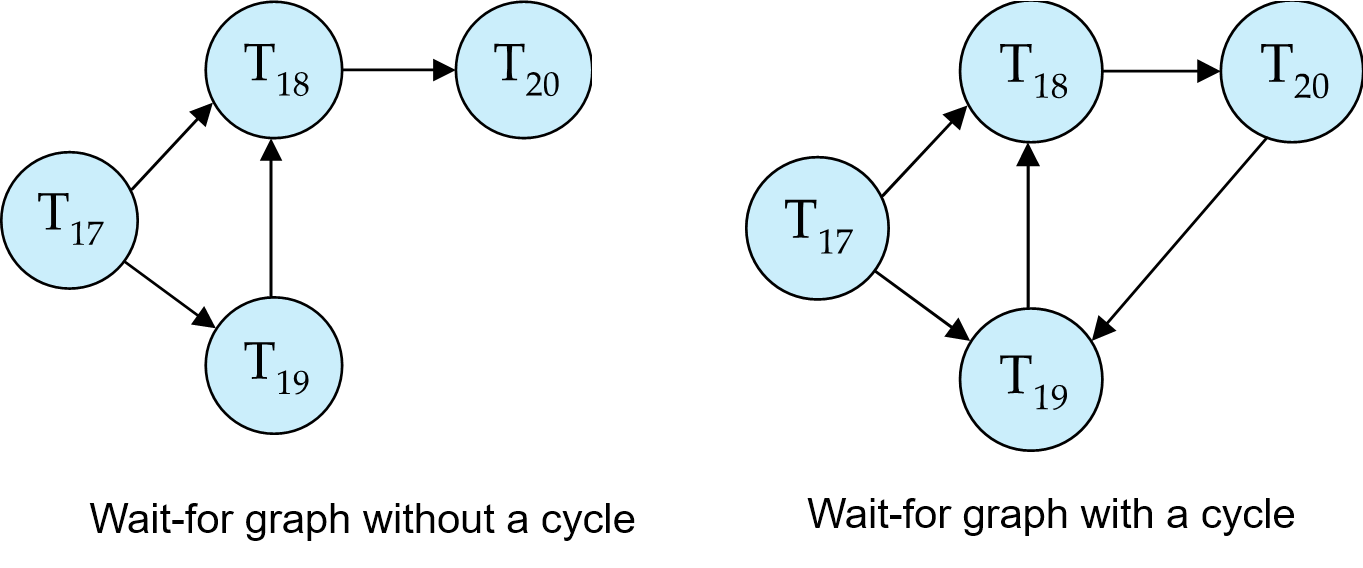
\includegraphics[width=0.6\linewidth]{fig/wait-for_graph.png}
\end{figure}

当事务$T_i$申请的数据项当前被$T_j$持有时,$T_i\to T_j$被插入图中。
只有当事务$T_j$不再持有事务$T_i$所需数据项时,这条边才从等待图删除。

当且仅当等待图存在环时,系统存在死锁。
要检测死锁,系统需要维护等待图,并周期性激活在等待图中搜索环的算法。

\subsubsection{死锁恢复}
通常做的动作有三个:
\begin{itemize}
	\item 选择牺牲者:决定回滚某一最小代价的事务
	\item 回滚:一旦确定回滚事务,则需确定该事务回滚多远,包括彻底回滚和部分回滚
	\item 饿死:如果选择牺牲者主要基于代价,则有可能同一事务总是被选为牺牲者,那该事务始终不能完成任务,就饿死(starvation)了
\end{itemize}

\subsection{基于时间戳的协议}
若事务$T_i$已赋予时间戳$TS(T_i)$,此时有一新事务$T_j$进入系统,则$TS(T_i)<TS(T_j)$,可利用\textbf{系统时钟}或者\textbf{逻辑计数器}实现。
事务的时间戳决定了串行化顺序,因此若$TS(T_i)<TS(T_j)$,则系统必须保证所产生的串行调度等价于事务$T_i$出现在事务$T_j$之前的某个串行调度。

\begin{itemize}
	\item 若$TS(T_i)\geq$W-timestamp(Q),则执行读操作
	\item 若$TS(T_i)\geq$R/W-timestamp(Q),则执行写操作
	\item 其他情况都会导致回滚
\end{itemize}
% !TEX root = main.tex

\section{恢复系统} % Chap 16
\subsection{故障分类}
\begin{itemize}
	\item 事务故障(failure)
	\begin{itemize}
		\item 逻辑错误:事务由于某些内部条件而无法继续正常执行,如非法输入。
		\item 系统错误:系统进入一种不良状态(如死锁),事务无法正常运行,但是之后某个时间点能够重新执行。
	\end{itemize}
	\item 系统崩溃(crash):硬件故障,或数据库软件/操作系统的漏洞,导致易失性存储器内容丢失,事务停止。
	\item 磁盘故障(failure):数据传送过程中由于磁头损坏或故障造成的磁盘块上内容丢失。
\end{itemize}

\subsection{恢复与原子性}
使用日志来重做(redo)和撤销(undo)事务。

事务回滚操作:
\begin{enumerate}
	\item 从后往前扫描日志,对于所发现的$T_i$的每个形如$<T_i,X_j,V_1,V_2>$的日志记录:
	\begin{enumerate}
		\item 值$V_1$被写到数据项$X_j$中,且
		\item 往日志中写一个特殊的只读日志记录$<T_i,X_j,V_1>$,其中$V_1$是在本次回滚中数据项$X_j$恢复成的值。这种日志称作补偿日志记录(compensation log record)。
	\end{enumerate}
	\item 一旦发现$<T_i,start>$的日志记录,就停止从后往前扫描,并往日志中写一个$<T_i,abort>$的日志记录
\end{enumerate}

\end{document}

% 1,2,3,4,6,7,8,10,11,14,15,16